\documentclass{article}


% if you need to pass options to natbib, use, e.g.:
%     \PassOptionsToPackage{numbers, compress}{natbib}
% before loading neurips_2022


% ready for submission
\usepackage[final]{neurips_2022}


% to compile a preprint version, e.g., for submission to arXiv, add add the
% [preprint] option:
%     \usepackage[preprint]{neurips_2022}


% to compile a camera-ready version, add the [final] option, e.g.:
%     \usepackage[final]{neurips_2022}


% to avoid loading the natbib package, add option nonatbib:
%    \usepackage[nonatbib]{neurips_2022}


\usepackage[utf8]{inputenc} % allow utf-8 input
\usepackage[T1]{fontenc}    % use 8-bit T1 fonts
\usepackage{hyperref}       % hyperlinks
\usepackage{url}            % simple URL typesetting
\usepackage{booktabs}       % professional-quality tables
\usepackage{amsfonts}       % blackboard math symbols
\usepackage{nicefrac}       % compact symbols for 1/2, etc.
\usepackage{microtype}      % microtypography
\usepackage{xcolor}         % colors
\usepackage{graphicx}
\usepackage{amsmath}
\usepackage{amsthm}
\usepackage{amssymb,amsfonts}
\usepackage{booktabs}
\usepackage{algorithm}
\usepackage{algorithmic}
\usepackage{color}
\usepackage{subcaption}
\usepackage{enumitem}
\usepackage{pifont}
\usepackage{mathtools}
\usepackage{arydshln}
\usepackage{multirow}
\usepackage{wrapfig}

\newcommand{\modelParamter}{\omega}
\newcommand{\horizon}{T_{H}}
\newcommand{\datapoint}{x}
\newcommand{\condition}{\boldsymbol{z}_{E}}
\newcommand{\state}{s}
\newcommand{\observation}{o}
\newcommand{\action}{a}
\newcommand{\transition}{t}
\newcommand{\reward}{r}
\newcommand{\agentIndex}{k}
\newcommand{\gameIndex}{j}
\newcommand{\quantielIndex}{i}
\newcommand{\dataset}{\mathcal{D}}
\newcommand{\expect}{\mathbb{E}}
\newcommand{\feature}{e}
\newcommand{\confidence}{c}
\newcommand{\error}{\epsilon}
\newcommand{\impact}{\phi}
\newcommand{\playerId}{l}
\newcommand{\constant}{C}
\newcommand{\splitnum}{m}
\newcommand{\sys}{RiGIM}
\newcommand{\bin}{B}
\newcommand{\goal}{g}
\newcommand{\system}{\sys\;}
\newtheorem{example}{Example}
\newtheorem{proposition}{Proposition}
\DeclareMathOperator*{\argmax}{argmax}


\title{Uncertainty-Aware Reinforcement Learning for Risk-Sensitive Player Evaluation in Sports Game}

\author{
Guiliang Liu$^{1,2,3}$, Yudong Luo$^{1,3}$, Oliver Schulte$^{4}$, Pascal Poupart$^{1,3}$ \\
${^1}$University of Waterloo, ${^2}$The Chinese
University of Hong Kong, Shenzhen,\\ 
${^3}$Vector Institute,
${^4}$Simon Fraser University\\
\texttt{liuguiliang@cuhk.edu.cn,yudong.luo@uwaterloo.ca},\\
\texttt{oschulte@cs.sfu.ca,ppoupart@uwaterloo.ca}
}

\begin{document}

\maketitle
%\vspace{-0.2in}
\begin{abstract}
%\vspace{-0.1in}
A major task of sports analytics is player evaluation. Previous methods commonly measured the impact of players' actions on desirable outcomes (e.g., goals or winning) without considering the risk induced by stochastic game dynamics.  In this paper, we design an uncertainty-aware Reinforcement Learning (RL) framework to learn a risk-sensitive player evaluation metric from stochastic game dynamics. To embed the risk of a player’s movements into the distribution of action-values, we model their 1) {\it aleatoric uncertainty}, which represents the intrinsic stochasticity in a sports game, and 2) {\it epistemic uncertainty}, which is due to a model's insufficient knowledge regarding Out-of-Distribution (OoD) samples. We demonstrate how a distributional Bellman operator and a feature-space density model can capture these uncertainties. Based on such uncertainty estimation, we propose a Risk-sensitive Game Impact Metric (RiGIM) that measures players' performance over a season by conditioning on a specific confidence level. Empirical evaluation, based on over 9M play-by-play ice hockey and soccer events, shows that RiGIM correlates highly with standard success measures and has a consistent risk sensitivity.
\end{abstract}
%\vspace{-0.1in}
\section{Introduction}
%\vspace{-0.05in}
The advancement of player tracking and object detection systems enables data-driven analytics for professional sports players. A common approach to evaluating the contribution of players is to quantify their action impacts.  Previous performance metrics~\cite{Routley2015Markov,Liu2018DRL,Decroos2019Actions,Luo2020IRL} computed the expected impact of an action on scoring or winning a game. However, actions with significantly different distributions of impact can have the same expectations. As a result, the expectation-based metrics cannot differentiate the risk-seeking actions from the risk-averse ones. How to distinguish these actions and assign proper credits to the players remains a fundamental challenge in sports analytics.

An important step toward a risk-sensitive evaluation metric is to model the distributions of action values. To achieve this goal, distributional Reinforcement Learning (RL)~\cite{bdr2022} predicts the supporting quantiles of action-value distributions. Previous distributional RL methods~\cite{bellemare2017distributional,Dabney2018DistributionalRL,Mavrin2019DistributionalRL,Zhou2020NonCrossing,Zhou2021Quantile} mainly studied the virtual environments with deterministic transitions (e.g., Atari~\cite{bellemare2013arcade} or Mujoco~\cite{Todorov2012Mujoco}), whereas sports games are real environments with stochastic game dynamics and complex context features. Moreover, player evaluation, as a data-driven task, requires learning from a fixed dataset without exploration. The model must be able to handle the distribution shift experienced at test time.

To mitigate the impact of distribution shift, Offline RL algorithms~\cite{Levine2020OfflineRL} typically strive for conservative policies that discourage visits to Out-of-Distribution (OoD) states by penalizing corresponding values. However, this approach cannot be scaled to player evaluation since 1) our goal is not control (i.e., improving players' policy), but to use RL as an analytical tool to evaluate observed actions in professional games, and 2) penalizing actions in OoD states distorts the evaluation.
%These conservative policies, however, cannot be applied to player evaluation, where RL acts as an analytic tool for evaluating players' movements in the dataset instead of controlling agents.


\begin{figure}
    \centering
    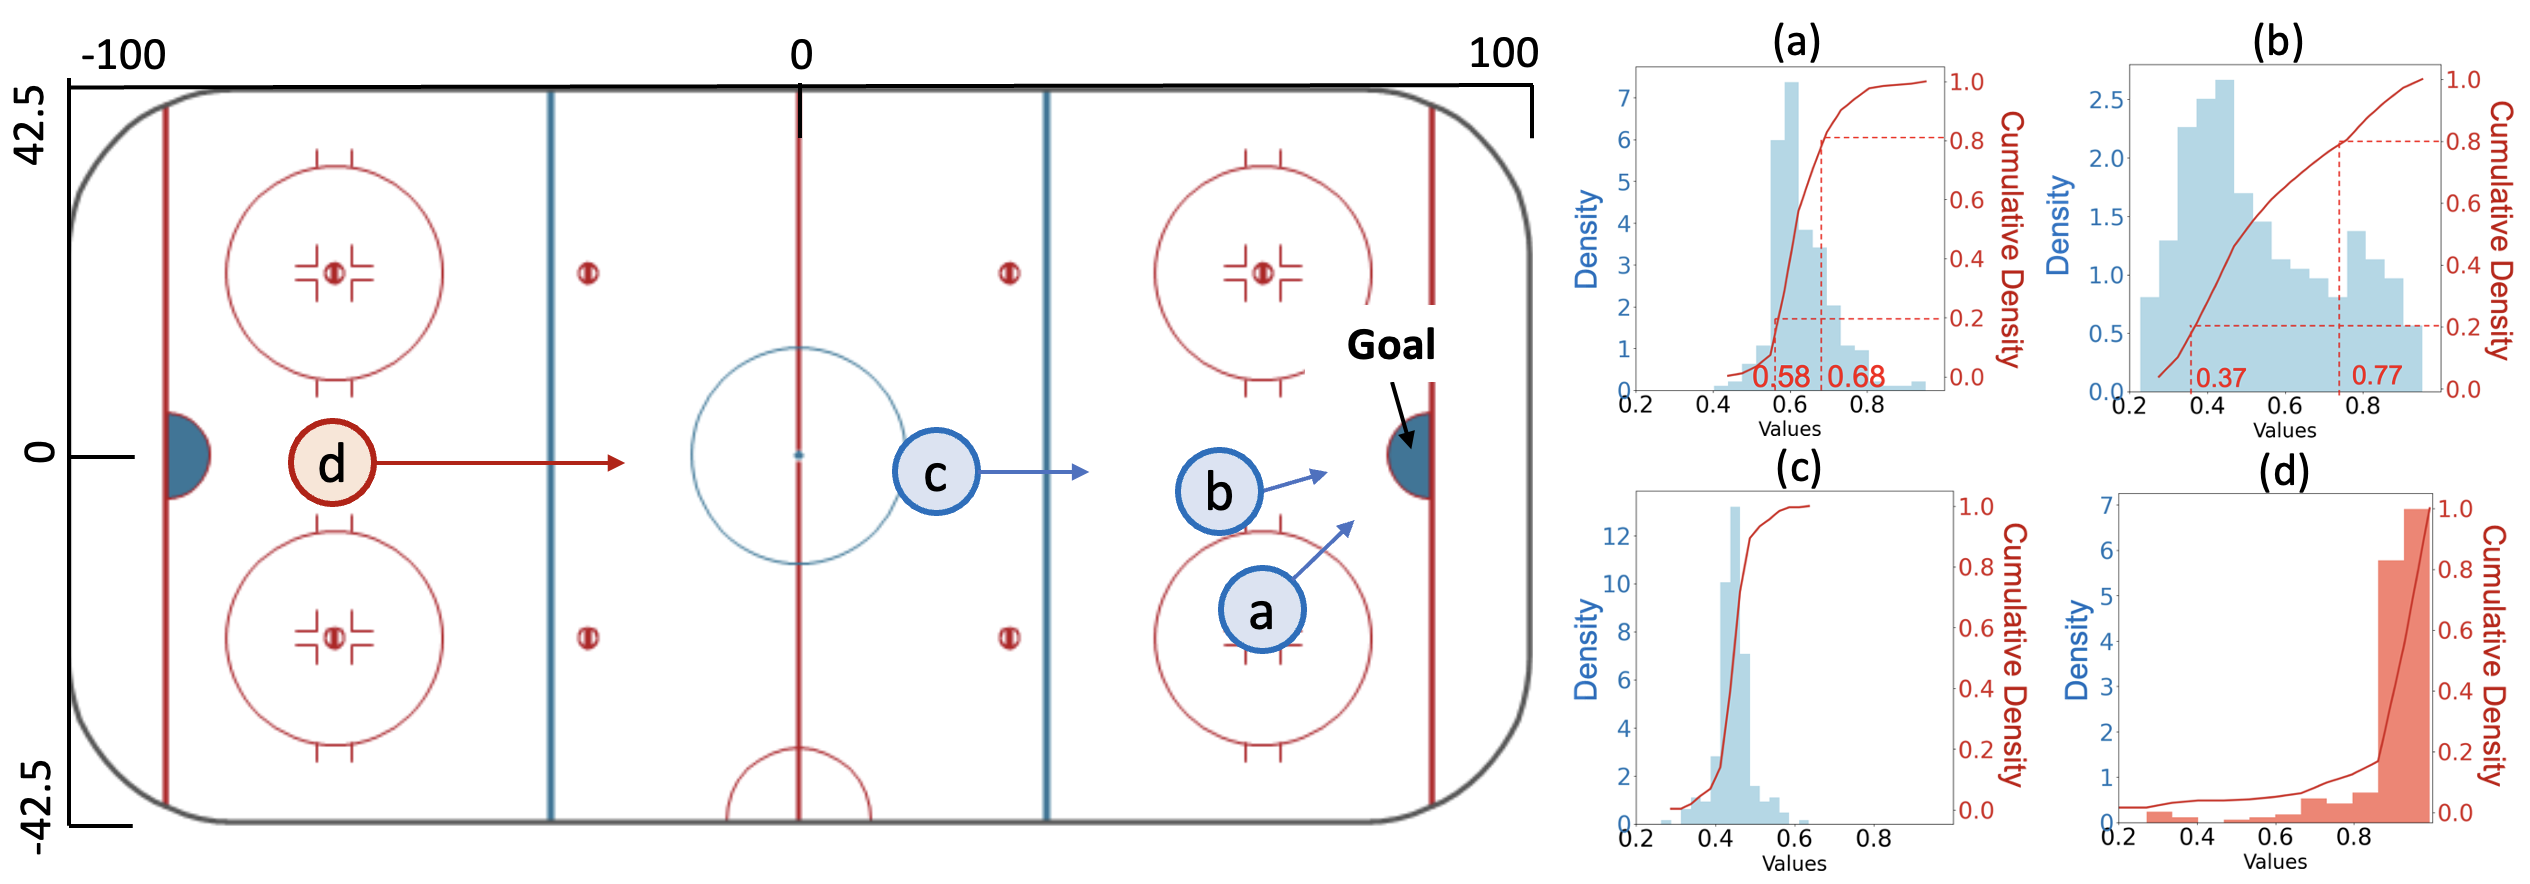
\includegraphics[scale=0.3]{figures/ice-hockey-rink-updated.png}
    % \begin{minipage}{0.5\textwidth}
    % \centering
    % 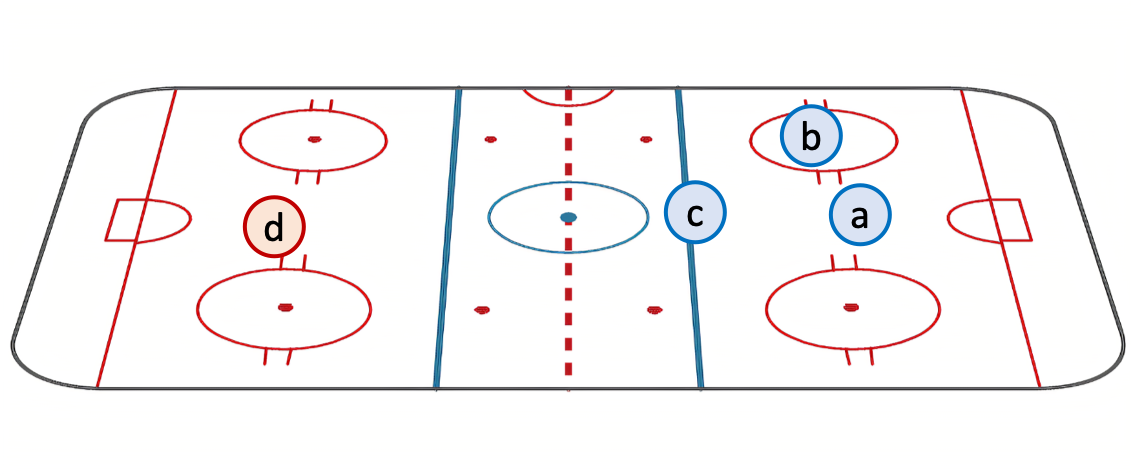
\includegraphics[scale=0.35]{figures/ice-hockey-view-marked.png}
    % \vspace{-0.15in}
    % \end{minipage}
    % \begin{minipage}{0.12\textwidth}
    % \centering
    % 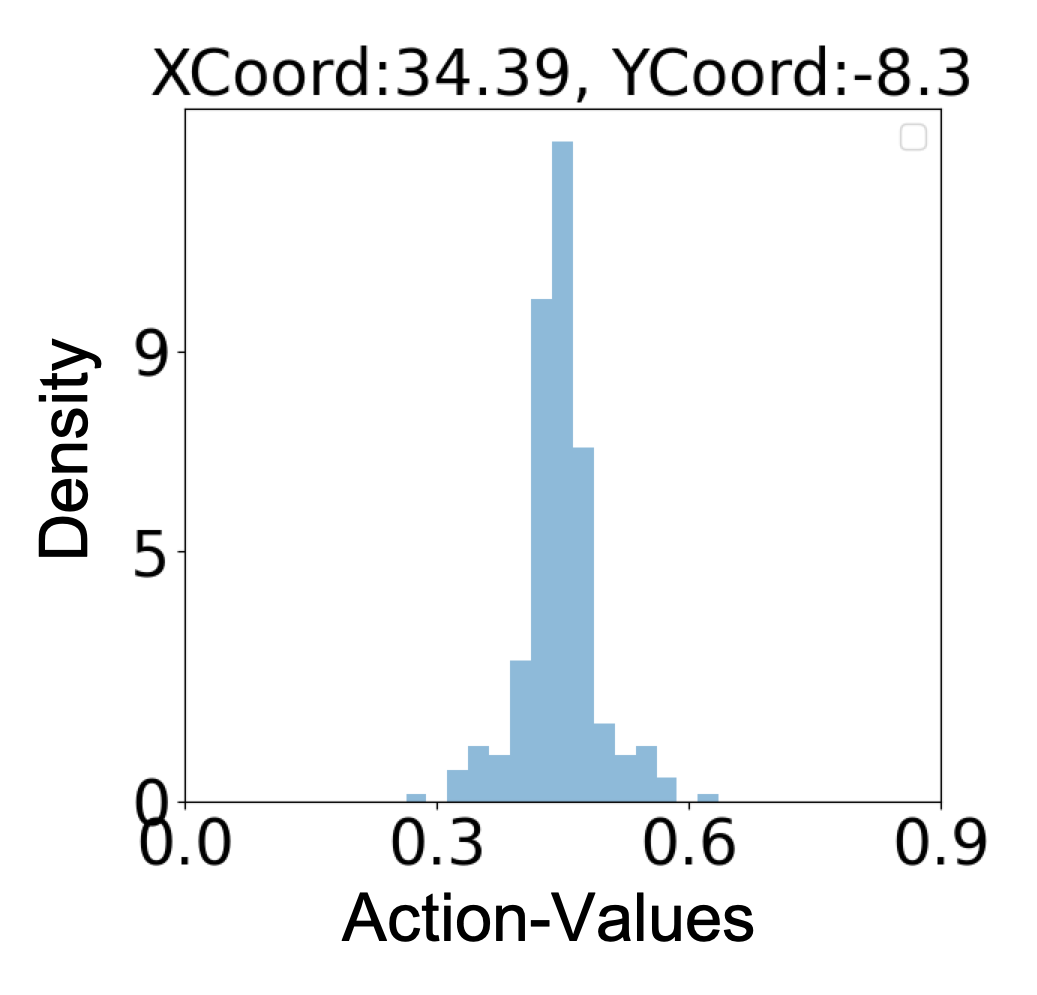
\includegraphics[scale=0.13]{figures/distribution_idx_2_XCoord_34.39_YCoord_-8.3-marked.png}
    % \end{minipage}\hfill
    % \begin{minipage}{0.12\textwidth}
    % 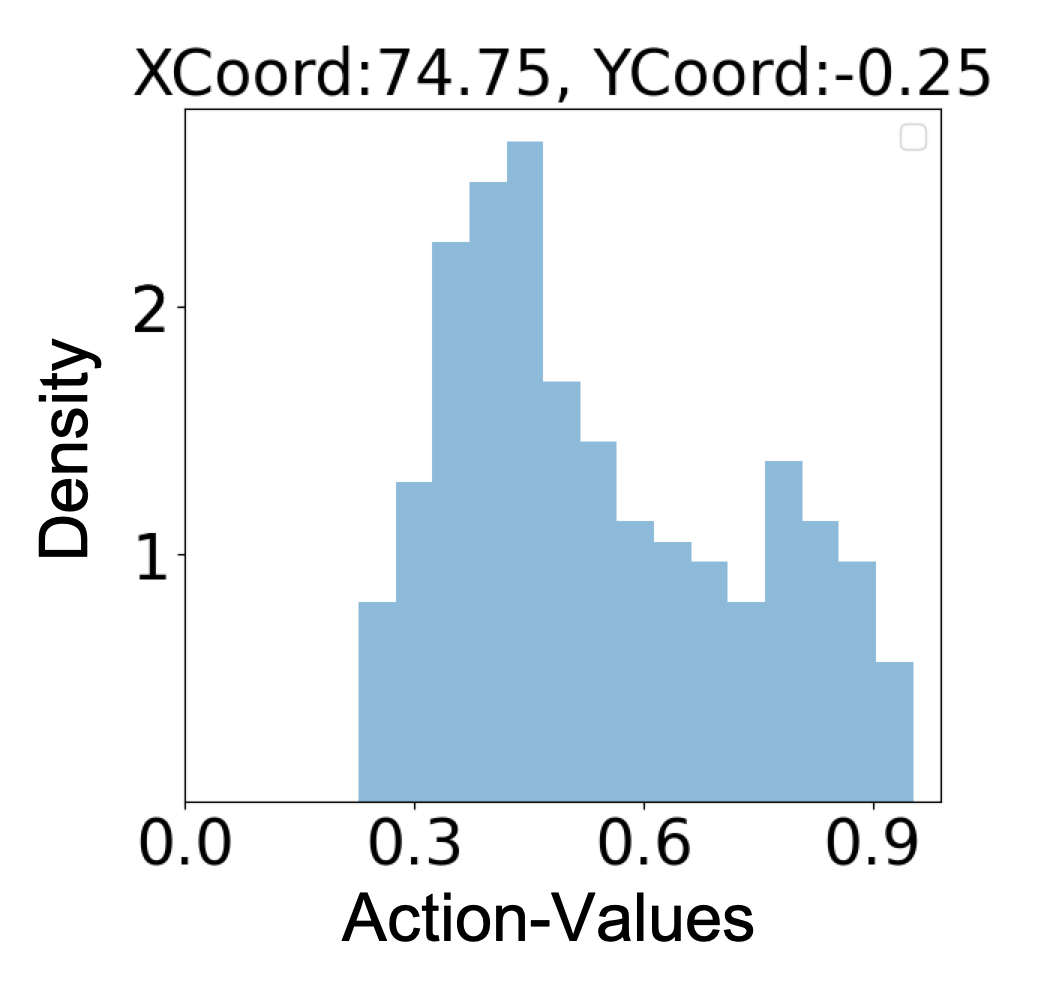
\includegraphics[scale=0.13]{figures/distribution_idx_21_XCoord_74.75_YCoord_-0.25-marked.png}
    % \end{minipage}\hfill
    % \begin{minipage}{0.12\textwidth}
    % 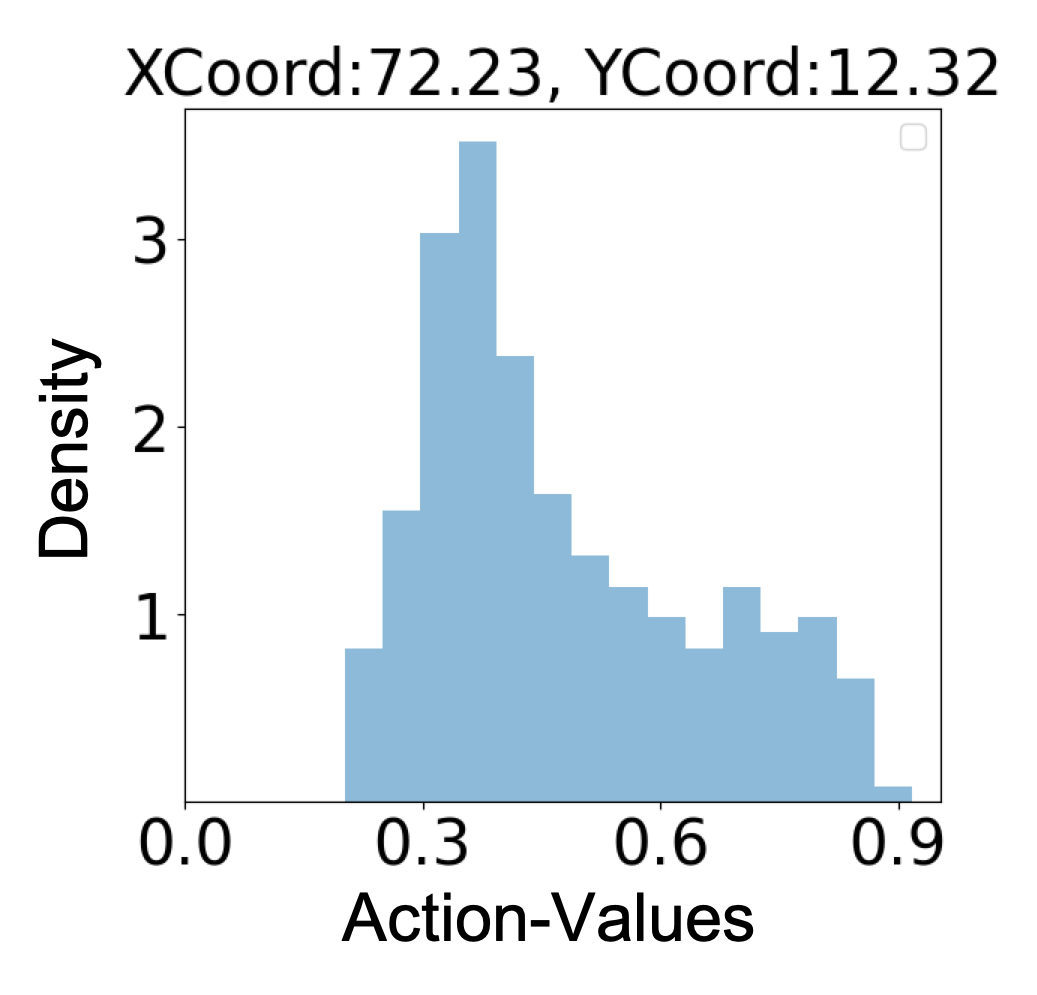
\includegraphics[scale=0.13]{figures/distribution_idx_22_XCoord_72.23_YCoord_12.32-marked.png}
    % \end{minipage}\hfill
    % \begin{minipage}{0.12\textwidth}
    % 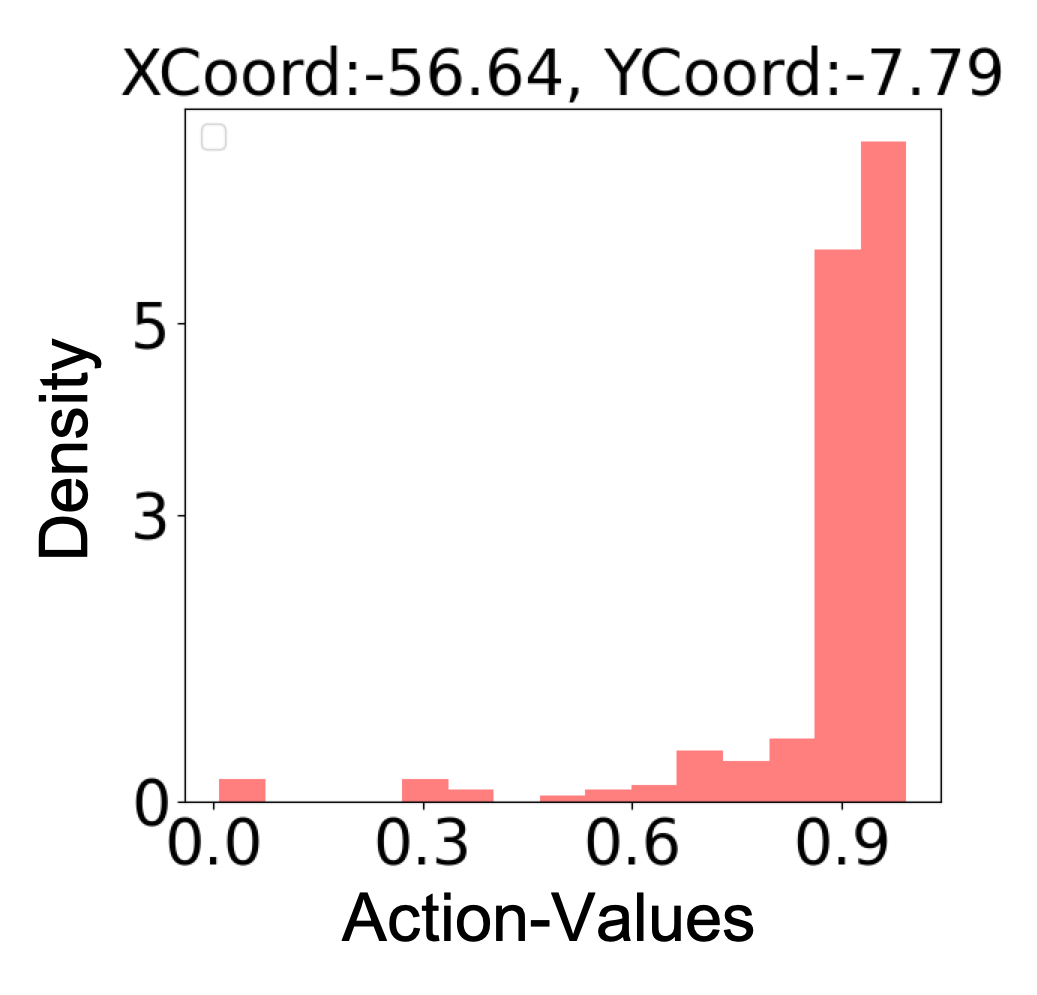
\includegraphics[scale=0.13]{figures/distribution_idx_35_XCoord_-56.64_YCoord_-7.79-marked.png}
    % \end{minipage}
    % \vspace{-0.1in}
    % \begin{minipage}{0.5\textwidth}
    % \centering
    % 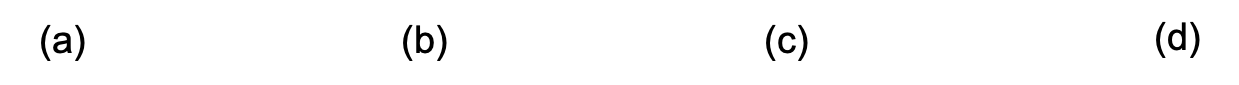
\includegraphics[scale=0.35]{figures/ice-hockey-view-label.png}
    % \end{minipage}
    % \vspace{-0.1in}
    % \begin{minipage}{0.4\textwidth}
    % 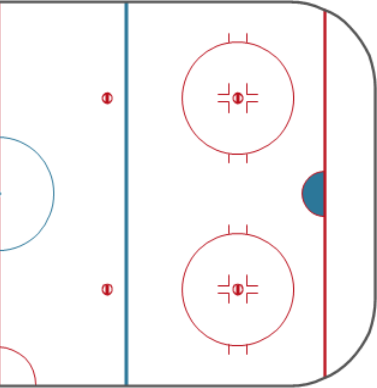
\includegraphics[scale=0.23]{figures/hockey-field-half.png}
    % \end{minipage}\hfill
    % \begin{minipage}{0.6\textwidth}
    %     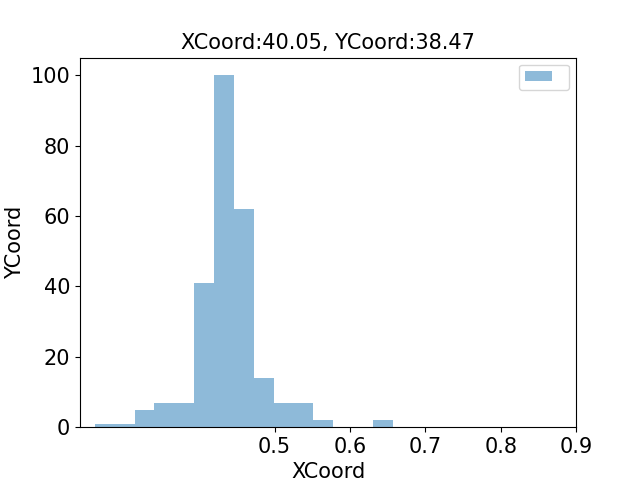
\includegraphics[scale=0.1]{figures/distrib_example_1_oct28.png}
    %     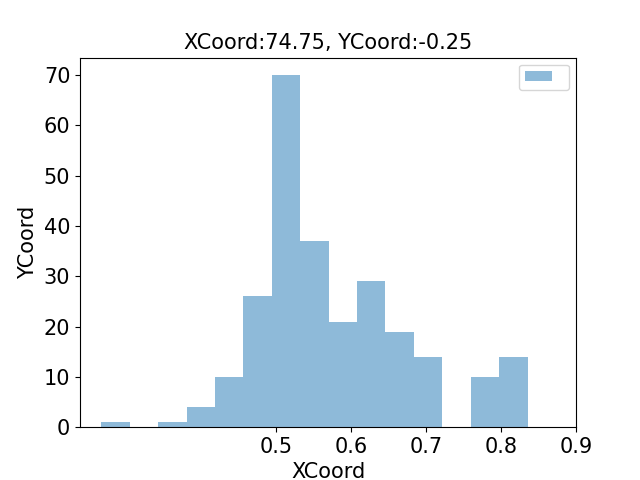
\includegraphics[scale=0.1]{figures/distrib_example_2_oct28.png}\\
    %     \includegraphics[scale=0.1]{figures/distrib_example_3_oct28.png}
    %     \includegraphics[scale=0.1]{figures/distrib_example_4_oct28.png}
    % \end{minipage}
    % \vspace{-0.15in}
    \caption{
    The predicted distribution of future goals in an ice hockey game between Blues and Coyotes, 2018-19 NHL season. The shots are made in the positions (a) - (d), providing important {\it motivations} for 1) {\bf risk-sensitive evaluation}: Distributions (a) and (b) have {\it the same expectation} (around 0.6), but the first shot has a larger risk-averse estimate (at the confidence $0.8$, we find $0.58 > 0.37$) and a smaller risk-seeking estimate (at the confidence $0.2$, we find $0.68 < 0.77$), and thus they have {\it different impact on risk-sensitive evaluation}. 2) {\bf Post-hoc calibration}: the event of shooting from the position (d) (the back-court) is rare in an ice hockey game, and thus this event is likely to be OoD, leading to a biased prediction at (d) (the predicted scoring chances are too large).
    % The ice hockey rink, where players shoot the puck to their opponent's goal (on the right) in a match between Blues and Coyotes, 2018-19 NHL season. For quantifying the aleatoric uncertainty, we predict the distributions of future goals for the shots in positions (a) - (d), but the prediction (d) should be filtered since it is OoD (shooting from the deep backcourt is rare) and thus is likely to be incorrect (the predicted scoring chances are too large).
    }
    \label{fig:examples-distribution-ice-hockey}
    \vspace{-0.15in}
\end{figure}

In this paper, we design an uncertainty-aware RL framework for risk-sensitive player evaluation. Figure~\ref{fig:examples-distribution-ice-hockey} shows a real-world example introducing our key motivations. Instead of directly influencing players' actions like other RL algorithms, we perform a post-hoc calibration of the learned action values. The main idea of our framework is to model important types of uncertainty in sports games: 

% \begin{itemize}[leftmargin=*]
%   \item 
1) {\it Aleatoric uncertainty} captures the intrinsic stochasticity of game dynamics caused by stochastic rewards, transition dynamics, and policies. We show that this stochasticity can be captured by a distributional Bellman operator and propagated between action-value distributions by implementing Temporal-Difference (TD) learning with distributional RL.
  
2) {\it Epistemic uncertainty} is due to the finite training samples and OoD state-action pairs during testing. Online RL algorithms can overcome this uncertainty given sufficient exploration in the environment~\cite{Mavrin2019DistributionalRL}. However, when we have only a demonstration dataset with limited samples, the influence of epistemic uncertainty cannot be ignored. Striving for simplicity and scalability, we model the epistemic uncertainty with a Feature-Space Conditional Normalizing Flow (FS-CNF).
% \end{itemize} 

Based on the uncertainty estimations, we develop a Risk-sensitive Game Impact Metric (RiGIM) for player evaluation. RiGIM filters the predictions for OoD samples and computes the impact of players' actions by conditioning on a confidence level.
% by following the Value-at-Risk (VaR) method~\cite{duffie1997overview}
Empirical evaluation shows that RiGIM is highly correlated with standard measures when compared to other baselines. 
We measure the accuracy of action-value predictions by matching them empirically with game results and evaluate the risk-sensitivity of \system by its correlations with standard measures at different confidence levels.

\noindent\textbf{Contributions.} 1) We design an uncertainty-aware RL framework that enables post-hoc calibrations on action values according to their aleatoric and epistemic uncertainties. 2) We demonstrate how the distributional Bellman operator captures the aleatoric uncertainty with action-value distributions from both a theoretical and an empirical perspective. 3) Striving for scalability, we design a feature-space density estimator that estimates the epistemic uncertainty with a minimum overhead. 4) To the best of our knowledge, RiGIM is the first risk-sensitive metric that incorporates the inherent risk in environment dynamics into player evaluation. Although this work mainly focus professional sports games, our method is general and can be scaled to other stochastic environments or domains.

%\vspace{-0.05in}
\section{Related Works}
%\vspace{-0.05in}
In this section, we introduce previous works that are most related to our approach.

\noindent\textbf{Uncertainty Estimation for RL.}
Uncertainty estimates have been widely used in RL for guiding exploration and stabilizing policies. To achieve this goal, an effective approach is to measure the uncertainty of {\it future returns}: ~\cite{ODonoghue2018UncertaintyBellman} designed an 
uncertainty Bellman equation that estimates the variance of the Q-value posterior distributions.
% ~\cite{wu2021UncertaintyActorCritic} proposed using Monte-Carlo drop-out to capture the uncertainty of action values.
Distributional RL methods ~\cite{bellemare2017distributional,Dabney2018DistributionalRL,Mavrin2019DistributionalRL,Zhou2020NonCrossing,Zhou2021Quantile,Tang2018DistribExplore,Zhang2019QUOTA,luo2022distributional} directly model the distribution of future returns by computing corresponding quantities.  Bootstrapped DQN methods ~\cite{Osband2016DeepBootstrapped,Chen2017QEnsembles,Osband2018RandomizedPrior,Silva2020UncertaintyActionAdvise} learn ensembles of action-value Q functions to capture uncertainty. Some following works~\cite{Kumar2019Stable,An2021OfflineQEnsemble} extend the Q-ensemble methods to offline RL settings by learning from a fixed dataset. Instead of focusing on the returns' uncertainty, an alternative approach is to measure the uncertainty of {\it model dynamics}: ~\cite{Yu2020MOPO,Kidambi2020MOReL} proposed model-based RL approaches that predict the uncertainty of dynamics models and penalize the actions leading to uncertain returns. Instead of separately capturing the epistemic and aleatoric uncertainties, these methods often quantify the overall uncertainty with a unified measure (e.g., variance or entropy). 

Another line of approaches that heavily relies on uncertainty estimates is Risk-Sensitive RL (RSRL)~\cite{mihatsch2002risk}. The RSRL agents avoid states with high costs by estimating a risk measure (e.g., variance, Value at Risk (VaR), or Conditional VaR~\cite{rockafellar2000optimization}). These algorithms~\cite{Shen2014RSRL,Chow2015RSRobust} often learn a controlling policy based on a known MDP instead of an offline dataset (with unknown dynamics). 

\noindent\textbf{Player Evaluation.} 
The most common approach to player evaluation is to quantify the impact of their actions on game results~\cite{schwartz2017handbook}. Previous works measured action impacts by predicting 1) whether a goal will be scored within a fixed look-ahead horizon~\cite{Decroos2019Actions}, 2) the change of winning chances~\cite{Xenopoulos2020CounterStrike}, and 3) the expected number of goals within a possession~\cite{cervone2016multiresolution}.  
Some recent works also trained action-value Q-functions by dynamic programming~\cite{Routley2015Markov}, deep Sarsa~\cite{Liu2018DRL,Liu2020soccer} and Inverse RL~\cite{Luo2020IRL}. These methods compute an expected action value without modeling their potential risk, and they commonly assume the training and testing datasets are identically distributed. 

% For the {\it online} RL problems where the agent can interact with the environment for collecting samples, the epistemic will shrink to zero when the agent learns the complete knowledge in the environment by running the exploration algorithm~\cite{Mavrin2019DistributionalRL,bellemare2017distributional}. In this case, the predictive uncertainty can directly captures the aleotoric uncertainty. However, for an {\it data-driven offline} RL problem (Section~\ref{subsec:offline-problem}), the training dataset is fixed and no exploration is allowed. The epistemic uncertainty cannot be eliminated since the environment commonly contains unexplored states and action by the demonstrate policy (with which $\dataset$ is collected). To develop an accurate value function for player evaluation, We must build separate model for capturing epistemic and aleotoric uncertainty.
% Unlike previous work that estimate uncertainty with complex approximation methods (e.g., variational model, ensemble models and Bayesian neural networks \textcolor{blue}{maybe add citation here}), in this work, we build deterministic model for capture uncertainty.
%\vspace{-0.05in}
\section{Uncertainty-Aware RL framework for Player Evaluation}
%\vspace{-0.05in}
We represent the dynamics in sports games with a Markov Game model and  introduce the motivation of estimating the aleatoric uncertainty and the epistemic uncertainty.
%\vspace{-0.05in}
\subsection{Finite-Horizon Markov Game Model}
%\vspace{-0.05in}
Player evaluation metrics commonly evaluate players by how much their actions influence the opportunity of scoring the next goal~\cite{Liu2018DRL,Decroos2019Actions,Sun2020Cracking}. Following this setting,  we divide a sports game into {\it goal-scoring episodes}, so that each episode 1) begins immediately after a goal (or at the beginning of the game), and 2) terminates when the next goal is scored (or the end of the game is reached). From an algorithmic perspective, this setting allows us to bound the support of future-goals distribution (Section~\ref{subsec:aleatoric-uncertainty}) into $[0,1]$,
% without discounting actions' impact on goals (e.g., rewards),
which leads to faster model convergence and more accurate evaluations. 

For a scoring episode of length $\horizon$, we model its dynamics with a finite-horizon Markov game model~\cite{Littman1994MarkovGame}$: G=(\mathcal{\MakeUppercase{\state}}, \boldsymbol{\mathcal{\MakeUppercase{\action}}}, P_{\mathcal{\MakeUppercase{\transition}}}, \boldsymbol{\MakeUppercase{\reward}}, \mathcal{\MakeUppercase{\observation}},\horizon,\gamma)$. 
% For the $\gameIndex^{th}$ episode in the training dataset $\dataset$, 
At a time step $t\in[0,\horizon]$, an agent $\agentIndex$ performs an action $\action_{\agentIndex,t} \in \mathcal{\MakeUppercase{\action}}_{\agentIndex}$ at a game state $\state_{t} \in \mathcal{\MakeUppercase{\state}}$ after receiving an observation $\observation_{t} \in \mathcal{\MakeUppercase{\observation}}$. 
This process generates the next state $\state_{t+1} \sim P_{\mathcal{\MakeUppercase{\transition}}}(\cdot|\state_t, \action_t)$ and a reward
$\reward_{k,t}=\MakeUppercase{\reward}_{\agentIndex}(\state_{t},\action_{\agentIndex,t})$. $\gamma$ is a discount factor.
In this paper, we consider two agents $\agentIndex\in\{Home, Away\}$ representing the home and away teams. The observed data $\dataset=[(\observation_1,\action_{\agentIndex,1},\boldsymbol{\reward}_{1}),(\observation_2,\action_{\agentIndex,2},\boldsymbol{\reward}_{2}),$ $\ldots,(\observation_t,\action_{\agentIndex,t},\boldsymbol{\reward}_{t}),\ldots]$ records the action $\action_{\agentIndex,t}$ performed by the team $\agentIndex$ who possesses the puck.  To alleviate the partial observability, a game state includes the game history: $\state_{t} := (\observation_t,\action_{t-1},\observation_{t-1},\ldots,\observation_{0})$. The reward $\boldsymbol{\reward}_{t}$ is a 1-of-2 indicator vector that specifies which team ($Home, Away$) scores. We assign zeros to $\boldsymbol{\reward}_{t}$ until a team scores at the end of an episode.%\vspace{-0.05in}
\subsection{Uncertainty-Aware RL for Player Evaluation}\label{subsec:offline-problem}
%\vspace{-0.05in}
\noindent\textbf{Learning from Offline Data.} As a data-driven behavior analytic tool, the player evaluation model assigns values to players' actions by learning from an offline dataset. Under this setting, previous works~\cite{Routley2015Markov,Liu2018DRL,Liu2020soccer,Decroos2019Actions} commonly assumed the training and testing datasets are sampled from the same underlying distribution. However, in practice, since the behaviors of players may change when some team members (especially core players or the coach) are traded or hired during a season, there is no guarantee that the visitation frequency of state-action pairs is consistent in different games. It is natural to assume a distributional shift between the games in the training and testing dataset: while the value function is trained under one distribution, it will be evaluated on a different distribution.

% We define the player evaluation task as an offline Reinforcement Learning (RL) problem~\cite{Levine2020OfflineRL}. Unlike classic RL agent that are trained and tested under the given environments, the offline RL agent learns from a fixed dataset $\dataset$ without interacting with the environment or collecting additional transitions using the behavior policy. This setting is consistent with the ice hockey application, where RL is applied as a data-driven analytics tool for
% professional players instead of controlling artificial agents. Under this setting, the agent must learn action-value functions with the dataset of training games and evaluate performance of the players in testing games. The fundamental challenge of Offline RL is distributional shift: while value function trained under one distribution, it
% will be evaluated on a different distribution, due to the change in both visited states and demonstration policies (implemented by different teams). To derive a promising player evaluation, the agent must be aware the uncertainty of predictions (especially for the Out-of Distribution (OoD) states).

\noindent\textbf{Calibration with Uncertainty.}
To alleviate the influence of distribution shift, offline RL algorithms~\cite{Levine2020OfflineRL} commonly discourage the visit to OoD state-action pairs by lowering their values~\cite{Kumar2020CQL} or penalising their rewards~\cite{Yu2020MOPO} or constraining the updated policy~\cite{Fujimoto2019OffPolicy,Kumar2019Stable}. However, to evaluate players' performance, RL is employed as a policy evaluation tool instead of controlling players. The trajectories in testing games correspond to observed players' actions that cannot be changed or influenced by penalties. Instead, we perform a post-hoc calibration of the predicted action values by modeling their {\it epistemic uncertainty}, which is due to a lack of knowledge about OoD samples, and thus the resulting model is uncertain about the returns (Section~\ref{subsec:epistemic-uncertainty}). Since our goal is to develop a risk-sensitive player evaluation metric, we estimate distributions of action values to model their {\it aleatoric uncertainty}, which is due to the intrinsic stochasticity in the game dynamics (Section~\ref{subsec:aleatoric-uncertainty}).
In practice, the quantification of aleatoric uncertainty can be influenced by the epistemic uncertainty of input samples, so we filter the OoD samples by utilizing our density estimator (Section~\ref{subsec:evaluation-metric}) .

% The uncertainty of actions for a testing sample $(\Tilde{\state},\Tilde{\action})$ can be factorized into both the {\it epistemic} and the {\it aleatoric} uncertainty,
% % ~\cite{Smith2018Uncertainty,Hullermeier2021uncertainty,Mukhoti2021Uncertainty}, 
% where
% % \begin{enumerate}[nosep]
% \setlist[itemize]{leftmargin=*}
% \begin{itemize}
% \setlength\itemsep{0em}
%     \item Aleatoric uncertainty is due to the intrinsic stochasticity in the dynamics of ice hockey games. Since the transition and reward functions of ice hockey games are stochastic, the expected goals carry uncertainty.
%     \item Epistemic uncertainty is due to the model's lack of knowledge about the data $(\Tilde{\state},\Tilde{\action})$ (i.e., $(\Tilde{\state},\Tilde{\action})$ is Out-of-Distributed), and thus, the model is uncertain about the returns.
% \end{itemize}
% As a result, apart from the epistemic uncertainty due to distribution shift, the aleatory uncertainty (due to stochastic game dynamic) must be captured in order to develop a robust evaluation metric. In this work

% In the rest of this paper, we introduce the approach to capture aleatoric and epistemic uncertainty (Section~\ref{Sec:action-value-function}) and to estimate a risk-sensitive player evaluation metric (Section~\ref{Sec:evaluation-metric}).


% \subsection{Distributional Reinforcement Learning}
% \subsection{Distributional RL for Player Evaluation}
% Our approach of deriving a uncertainty-aware player evaluation metric is shown in Figure~xxx. We utilize distributional RL to learn an action-value function $Z(\state,\action)$ that predicts the distribution of expected future goals when a player perform an action $\action$ under a state $\state$. This distribution capture both the (partial\footnote{The distribution RL model might not capture the full epistemic uncertainty due to features collapse~\cite{Amersfoort2020Uncertainty}.}) {\it epistemic uncertainty} (induced by the OoD inputs $\state$ or $\action$ ) and the {\it aleatoric uncertainty} (induced by the stochasticity in environment dynamics)~\cite{Hullermeier2021uncertainty} of the player movement. We argue when measuring the risk of a player movement, only the aleotoric uncertainty should be counted (see Section~xxx). Based on samples from the predicted distribution, we compute a Vaule-at-Risk (VaR) Goal Impact metric  to value each player, based on the aggregated impact of their actions.
%\vspace{-0.05in}
\section{Modelling the Uncertainty of Action Values }\label{Sec:action-value-function}
%\vspace{-0.05in}
The aforementioned uncertainty-aware RL framework requires estimating the aleatoric and epistemic uncertainty for a risk-sensitive player evaluation. In this section, we introduce our distributional-RL approach for modelling aleatoric uncertainty and a feature-space density estimator for measuring epistemic uncertainty (Figure~\ref{fig:model-architecture} shows the model architecture).
% . Previous works demonstrate discriminate model and density 
% introduce how the our distributional-RL model and feature-space density estimator capture the aleatoric and epistemic uncertainty.
\begin{figure}[htbp]
\vspace{-0.15in}
\begin{minipage}[t]{0.51\textwidth}
    \hspace{-0.25in}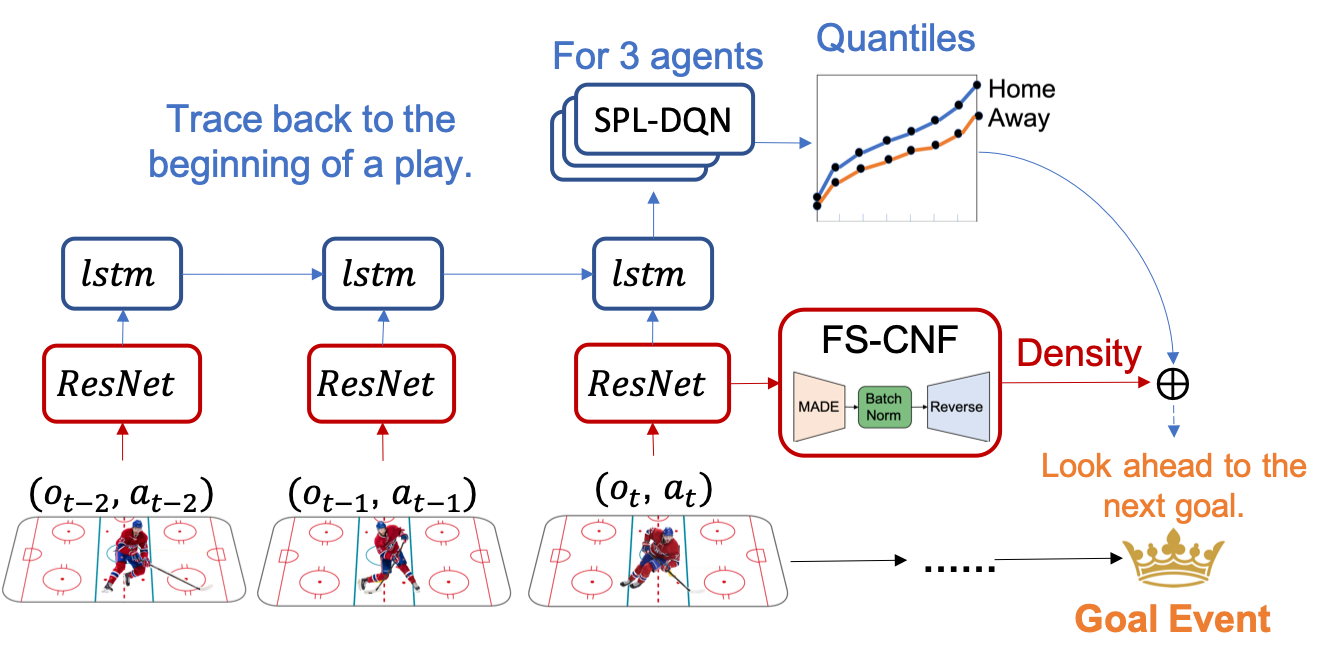
\includegraphics[scale=0.35]{figures/ice-hockey-net.png}
    \captionsetup{width=.95\linewidth}
    \caption{Model architecture. A play is a turn where one team attacks and the other defends. We add Spectral Normalization to ResNet outputs.}
    \label{fig:model-architecture}
\end{minipage}%
\begin{minipage}[t]{0.49\textwidth}
    \centering
    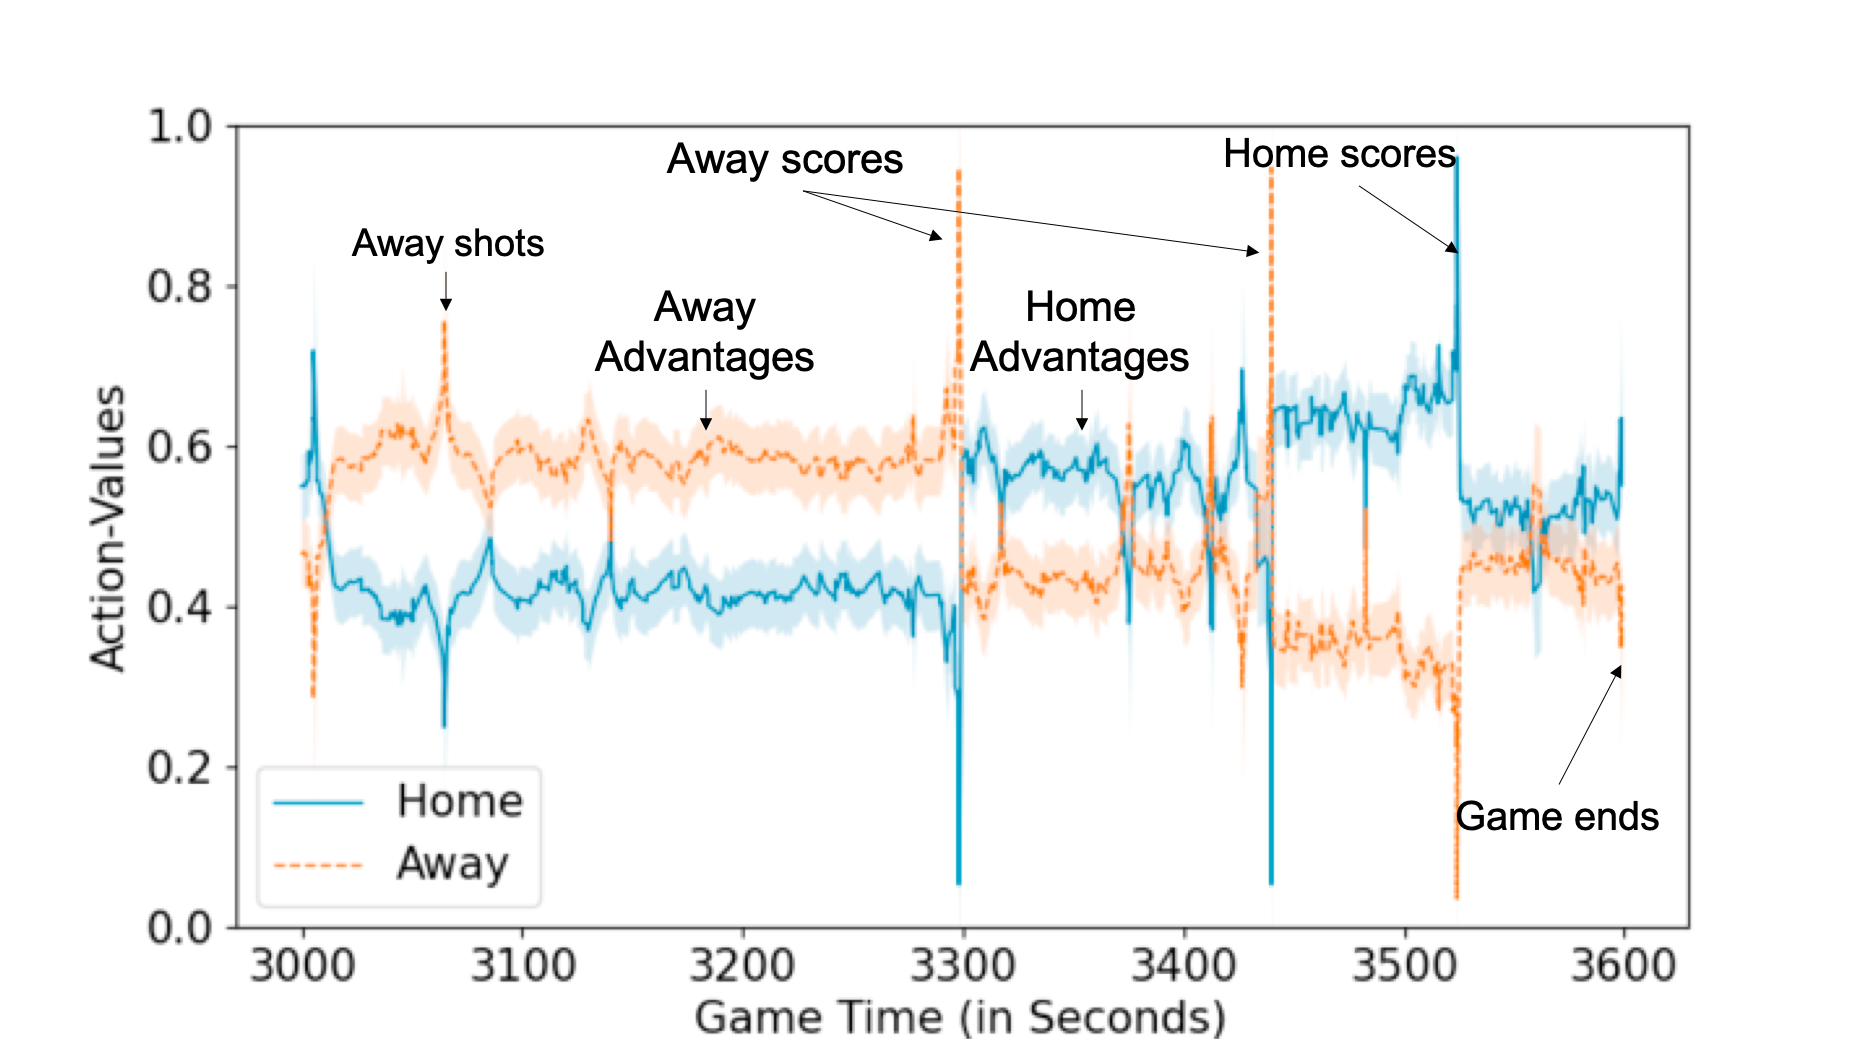
\includegraphics[scale=0.24]{figures/temporal-visualization-marked.png}
    \captionsetup{width=.95\linewidth}
    \caption{Illustrating the predicted distributions by showing the corresponding mean $\pm$ standard deviation at each time step in a sports game.}
    \label{fig:temporal-plot}
\end{minipage}
\vspace{-0.2in}
\end{figure}
% \subsection{Distribution Function for Action Values}
\subsection{Distributional RL for Capturing Aleatoric Uncertainty}\label{subsec:aleatoric-uncertainty}
Distributional RL learns the distribution of the random variable $Z_{\agentIndex}(\state_{t},\action_{t})$ that 
% \in P(\mathbb{R})^{\mathcal{\MakeUppercase{\action}}\times\mathcal{\MakeUppercase{\state}}}$ 
corresponds to the number of future goals when a player of team $k$ performs action $\action_{t}$ in state $\state_{t}$.  In other words, we can think of $Z_{\agentIndex}(\state_{t},\action_{t})$ as a random variable with outcomes corresponding to the sum of discounted rewards $\sum_{\iota=t}^{\horizon}\gamma^{\iota}\MakeUppercase{R}_{\agentIndex,\iota}(\MakeUppercase{\state}_\iota,\MakeUppercase{\action}_\iota)$, where $\MakeUppercase{\state}_\iota=\state_{\iota}$, $\MakeUppercase{\action}_\iota=\action_{\iota}$,
% $\reward_{\agentIndex,t}= \MakeUppercase{\reward}_{\agentIndex}(\state_{t},\action_{t})$, 
$\MakeUppercase{\state}_{\iota+1}$ is distributed according to $P_{\mathcal{\MakeUppercase{\transition}}}(\cdot|\MakeUppercase{\state}_\iota,\MakeUppercase{\action}_\iota)$ and $\MakeUppercase{\action}_\iota$ is distributed according to $\pi(\cdot|\MakeUppercase{\state}_\iota)$. 
% We use $T_{g}$ to denote the time step when the current goal-scoring episodes ends.
Following the Quantile-Regression (QR)-DQN method~\cite{bellemare2017distributional}, we represent the distribution of $Z$ by a uniform mixture of $N$ supporting quantiles by
$
\hat{Z}_{\agentIndex}(\state_{t},\action_{t}) = \frac{1}{N}\sum_{\quantielIndex=1}^N \delta_{\theta_{\agentIndex,\quantielIndex}(\state_{t},\action_{t})}$, where $\theta_{\agentIndex,\quantielIndex}$ estimates the quantile at the quantile level (or quantile index) $\hat{\tau}_i=\frac{\tau_{\quantielIndex-1}+\tau_\quantielIndex}{2}$ ($1\leq \quantielIndex\leq N$, and $\tau_\quantielIndex=\quantielIndex/N$) and  $\delta_{\theta_{\agentIndex,i}}$ denotes a Dirac distribution at $\theta_{\agentIndex,\quantielIndex}$. The model outputs [$\theta_{\agentIndex,1},\dots,\theta_{\agentIndex,N}$] are monotonically increasing quantile values computed with the spline DQN (SPL-DQN) by following~\cite{luo2022distributional}.
% Since $\hat{Z}_{\agentIndex}$ is defined in a scoring episode, the support of predicted action-value distributions is in $[0,1]$.


% \end{enumerate}
% We provide a uncertainty model for ice hockey games as follows:
% \vspace{-0.15in}
% \begin{align}
%     ~\label{eqn:uncertainty}\\
%      H(Z|\Tilde{\state},\Tilde{\action},\dataset) = I(Z;\modelParamter|\Tilde{\state},\Tilde{\action},\dataset) + \expect_{ p(\modelParamter|\dataset)}(H(Z|\modelParamter,\Tilde{\state},\Tilde{\action}))\nonumber
% \end{align}
% where the mutual entropy  $I(Z;\modelParamter|\Tilde{\state},\Tilde{\action},\dataset)$ measures the amount of information we would gain about the model parameters $\modelParamter$ if we were to observe a new point data $\Tilde{\state},\Tilde{\action}$. When the information gain is large, $\Tilde{\state},\Tilde{\action}$ is OoD and our model has a poor knowledge about this situation. $\expect_{p(\modelParamter|\dataset)}(H(Z|\modelParamter,\Tilde{\state},\Tilde{\action}))$ acts as a Bayesian model for predictions. $p(\modelParamter|\dataset)$ forms an approximation to the distribution of sports dynamics and thus capture their intrinsic stochasticity.

% \subsection{Uncertainty Modelling with Value Function}
\paragraph{Distributional Bellman Operator.}
When the player of a team $\agentIndex$ performs an action $\action_t$
% \sim\pi(\MakeUppercase{\action}_{t}|\MakeUppercase{\state}_{t}=\state_{t})$ 
at a state $\state_t$, the agent receives a reward $\MakeUppercase{\reward}_{\agentIndex}(\state_t,\action_t)$ and moves to a future state $\state_{t+1}\sim P_{\mathcal{\MakeUppercase{\transition}}}(\MakeUppercase{\state}_{t+1}|\state_t,\action_t)$ where the agent's next action $\action_{t+1}\sim\pi(\MakeUppercase{\action}_{t+1}|\MakeUppercase{\state}_{t+1})$. This stochastic process can be captured by a distributional Bellman operator $\mathcal{T}^{\pi}$~\cite{bellemare2017distributional}:
%\vspace{-0.1in}
\begin{equation}
    \mathcal{T}^{\pi}{Z}_{\agentIndex}(\state_t,\action_t) \overset{\Delta}{:=} \MakeUppercase{\reward}_{\agentIndex}(\state_t,\action_t) + \gamma {Z}_{\agentIndex}(\MakeUppercase{\state}_{t+1},\MakeUppercase{\action}_{t+1})~\label{eqn:bellman-operator}
    % \vspace{-0.05in}
\end{equation}
% where $\MakeUppercase{\state}^{\prime}$ and $\MakeUppercase{\action}$ are distributed according to $P(\cdot|\state,\action)$ and $ \pi_{\agentIndex}(\cdot|\MakeUppercase{\state}^{\prime})$. 
where $X\overset{\Delta}{:=}Y$ indicates that random variables $X$ and $Y$ follow the same distribution.
% Unlike $Q$-learning that estimate the expect value $\expect[Z^{\pi}(\state,\action)]$, distributional RL directly models the full distribution of $Z^{\pi}_{\agentIndex}$ to captures the uncertainty.
Based on the distributional Bellman operator, we estimate the supporting quantiles of $Z$ by minimizing the quantile Huber loss (with threshold $\eta$):
%\vspace{-0.05in}
\begin{align}
    \frac{1}{N}\sum_{\quantielIndex=1}^N\sum_{\quantielIndex^{\prime}=1}^N\rho^{\eta}_{\hat{\tau}_\quantielIndex}(\reward+\gamma\theta_{\quantielIndex^{\prime},\agentIndex}(\state_{t+1},\action_{t+1})-\theta_{\quantielIndex,\agentIndex}(\state_{t},\action_{t})) \text{ where }\nonumber~\label{eq:huber}
\end{align}%\vspace{-0.2in}
\begin{align}
    \begin{split}
    \rho_{\tau}^{\eta}(\sigma) = |\tau - \mathbb{I}_{\sigma<0}|\mathcal{L}_{\eta}(\sigma)~\text{ with }
    \mathcal{L}_{\eta}(\sigma) = \begin{cases}
    \tfrac12 \sigma^2, & |\sigma| \leq \eta\\
    \eta(|\sigma|-\frac12 \eta), & \mathrm{otherwise}.
\end{cases}
\end{split}
%\vspace{-0.05in}
\end{align}

{\it Illustration of Temporal Projection}. Figure~\ref{fig:temporal-plot} illustrates the mean $\pm$ standard deviation of the action-values sampled from the predicted distributions $\hat{Z}(\state,\action)$, where $\state$ and $\action$ follow the players' movements in a match between the Flyers (Home team) and the Maple Leafs (Away team) on March 15, 2019. The figure plots values
of the two output nodes. We highlight critical events and
match contexts to show the context-sensitivity of our predictions. 

We show that the predicted distribution of action values can measure the aleatoric uncertainty.

\begin{proposition}
Assume the Bellman consistency holds by $\hat{\boldsymbol{Z}} \overset{\Delta}{:=} \MakeUppercase{\boldsymbol{\reward}} + \gamma \boldsymbol{P}^{\pi}\hat{\boldsymbol{Z}}$ 
where $\hat{\boldsymbol{Z}}$, $\boldsymbol{\MakeUppercase{\reward}}$ are vector-valued random variables and $\boldsymbol{P}^{\pi}$ is the transition matrix of the stationary policy $\pi$, so $P^{\pi}_{(\state,\action),(\state^{\prime},\action^{\prime})}=P(\state^{\prime}|\action,\state)\pi(\action^{\prime}|\state^{\prime})$, the uncertainty of action-value distributions $\hat{\boldsymbol{Z}}$ under an entropy measure $H(\cdot)$ can be given by:
\begin{align}
    H(\hat{\boldsymbol{Z}}) = H[\boldsymbol{\MakeUppercase{\reward}}]-|\mathcal{\MakeUppercase{\action}}||\mathcal{\MakeUppercase{\state}}|\log(1-\gamma)+\log|\text{det}(\mathbf{d}^{\pi})|
\end{align}
where $\mathbf{d}^{\pi}=(1-\gamma)(I-\gamma \boldsymbol{P}^{\pi})^{-1}\in[0,1]^{|\MakeUppercase{\state}||\MakeUppercase{\action}|\times|\MakeUppercase{\state}||\MakeUppercase{\action}|}$ is the induced matrix for distributions over state-action tuples by following policy $\pi$ and transition $P_{\mathcal{\MakeUppercase{t}}}$. 
\end{proposition}

The proof is in Appendix B.1. Proposition 1 disentangles the entropy of $\boldsymbol{Z}$ into 1) the entropy of reward variables that quantifies the uncertainty of current rewards, 2) the uncertainty induced by the discount factor, which determines how much the current uncertainty estimation should be influenced by the stochasticity of future rewards or transitions (i.e., a small $\gamma$ reduces this influence), and 3) a log-absolute determinant of the induced distribution matrix, which measures the amount of stretch or change that the transition function $P_{\mathcal{\MakeUppercase{\transition}}}$ and the policy $\pi$ apply to the initial state-action distribution.
% factor by which the function expands or shrinks volumes near

Proposition 1 demonstrates that the key components for representing the aleatoric uncertainty can be captured by $Z$ when the Bellman consistency is reached by learning, which suggests the action-value distribution learned by distributional RL is an ideal estimator for aleatoric uncertainty.  However, in practice,  the estimation of $Z$ cannot be well generalized to all samples because of insufficient exploration or limited training data, so we need to estimate their epistemic uncertainty. 


% \begin{proposition}
% Assume the Bellman consistency holds by $\hat{Z}(\state_t,\action_t) \overset{\Delta}{:=} \MakeUppercase{\reward}(\state_t,\action_t) + \gamma \hat{Z}(\MakeUppercase{\state}_{t+1},\action_{t+1})$ 
% where $\MakeUppercase{\state}_{t+1}$ follows $ P_{\mathcal{\MakeUppercase{\transition}}}(\cdot|\state_{t},\action_{t})$ and
% % and ${\action}_{t+1}\sim\pi(\cdot|\MakeUppercase{\state}_{t+1})$
% ${\action}_{t+1}=\argmax_{\action_{t+1}} \expect_{P_{\mathcal{\MakeUppercase{\transition}}},\MakeUppercase{\reward}}[\hat{Z}(\state_{t+1}, \action_{t+1})]$
% , let $\hat{Z}(\state_{t},\action_{t};\dataset)$ be the distribution function learned by the training dataset $\dataset$ and let $\gamma=1$, the uncertainty capture by the predicted distribution under an entropy measure $H(\cdot)$ in a MDP with a finite horizon $\horizon$ is given by:
% \begin{align}
%     & H[Z(\state_{t},\action_{t};\dataset)]=(\horizon-t)\cdot\sum_{\Tilde{\state},\Tilde{\action}}\hat{d}_{{\state}_{t},{\action}_{t}}^{\pi}(\Tilde{\state},\Tilde{\action};\dataset)H(\MakeUppercase{\state}^{\prime}|\Tilde{\state},\Tilde{\action})\nonumber
%     % & \text{and } \phi(\Tilde{\state},\Tilde{\action};\dataset)=H(\MakeUppercase{\state}^{\prime}|\Tilde{\state},\Tilde{\action};\dataset) + H(\MakeUppercase{\action}^{\prime}|\MakeUppercase{\state}^{\prime},\Tilde{\state},\Tilde{\action};\dataset)
% \end{align}
% where $H[Z(\cdot)]$ denotes the entropy of predicted distribution and $\hat{d}_{{\state}_{t},{\action}_{t}}^{\pi}(\Tilde{\state},\Tilde{\action};\dataset)$ denotes the probability of visiting state-action pair $(\Tilde{\state},\Tilde{\action})$ from $({\state}_{t},{\action}_{t})$ within $(\horizon-t)$ steps.
% \end{proposition}

% The proof is in Appendix~\textcolor{blue}{xx}. Note that we define a deterministic reward function (so $H(\MakeUppercase{\reward})=0$). 
% % and the entropy of reward variable given a state-action pair is zero. 
% A stochastic reward function adds complexity to proof since $H(\MakeUppercase{\reward}+Z(\cdot))\leq H(\MakeUppercase{\reward})+H(Z(\cdot))$. This upper bound could be loose \textcolor{blue}{(depending on the assumptions of their parametric distributions.)} and the equivalence holds only when $H(\MakeUppercase{\reward})=0$ or $H(Z(\cdot))=0$.

% Proposition 1 shows that the intrinsic stochasticity in the environment for a given sample $(\Tilde{\state},\Tilde{\action})$ (denoted as $H(\MakeUppercase{\state}^{\prime}|\Tilde{\state},\Tilde{\action})$) can be captured by the predicted distribution of $Z|_{\state_{t},\action_{t}}$. However, the estimation of visiting probability
% % , entropy terms are 
% is based on training data $\dataset$ while the true visiting probability $d^{*}_{\state_t,\action_t}(\cdot)$ 
% % and entropy $\phi^{*}(\cdot)$ 
% follows the testing policy. 
% For a testing sample $(\Tilde{\state},\Tilde{\action})$ with small a density on the training distribution, it is difficult to drive an accurate estimation of entropy due to the lack of exploration. 
% The aleatoric uncertainty could be influenced by the epistemic uncertainty of $(\Tilde{\state},\Tilde{\action})$.


% Distributional RL directly predicts the distribution of discounted future goal $Z$ whose range is $[0, 1]$. Given a new data point $\Tilde{\state},\Tilde{\action}$, we can calculate its (approximated) predictive uncertainty $H(Z|\Tilde{\state},\Tilde{\action},\dataset)$ ($H(\cdot)$ indicates entropy) with the samples [$\theta_{1},\dots,\theta_{N}$]~\footnote{The sampling method is Inverse Transform Sampling.} from $p(Z)$. 

%\vspace{-0.05in}
\subsection{Density Estimator for Capturing Epistemic Uncertainty}\label{subsec:epistemic-uncertainty}
%\vspace{-0.05in}
By definition, epistemic uncertainty stems from limited training data and is inherent to the model fitting these data. A common measure of epistemic uncertainty is $I(\theta; y|\datapoint,\dataset)$~\cite{Smith2018Uncertainty,Amersfoort2020Uncertainty,Mukhoti2021Uncertainty}: the amount of information gained when the model $\theta$ observes the true label $y$ of an input $\datapoint$.
% (i.e., being uncertain about the data implies that the label can provide extra information to the model). 
To estimate this uncertainty measure, previous works~\cite{Lakshminarayanan2017Ensembles,Wen2020BatchEnsemble,Dusenberry2020Bayesian} utilized deep ensemble models and treated each ensemble as a sample from the posterior $p(\theta|\dataset)$. However, adding additional deep ensemble layers to a distributional RL model (i.e., as a {\it unified} estimator for the joint distribution $p(Z_{1,\dots,\MakeUppercase{\agentIndex}},\Theta|\dataset)$) significantly increases the model complexity. Striving for model simplicity and scalability for large datasets,  we build a feature space density estimator~\cite{Mukhoti2021Uncertainty} to detect OoD samples. 

In this work, we design a Feature Space Conditional Normalizing Flow (FS-CNF) to estimate sample density in the training distribution with a minimum overhead. The main components are:

\noindent\textbf{Feature Extractor.} FS-CNF shares the same feature extracting layers with the distributional RL models. 
Note that a common reason why traditional feature extractors might fail to capture epistemic uncertainty is feature collapse~\cite{Amersfoort2020FeatureCollapse}, which maps OoD samples to iD regions in feature space. To prevent this phenomenon, an ideal feature extractor $f_{\theta}$ must be subjected to a bi-Lipschitz constraint:
\begin{align}
\beta_{1}\|\datapoint_{1}-\datapoint_{2}\|_{I}\geq\|f_{\theta}(\datapoint_{1})-f_{\theta}(\datapoint_{2})\|_{F}\geq\beta_{2}\|\datapoint_{1}-\datapoint_{2}\|_{I}\text{ }\forall{\datapoint_{1},\datapoint_{2}\in\dataset}
\end{align}
where 1) the lower Lipschitz bound ensures sensitivity to distances in the input space (i.e., sensitive to OoD samples) and 2) the upper Lipschitz bound ensures smoothness in the feature space (i.e., prevents overfitting to the input variations). To ensure this bi-Lipschitz condition in practice, we follow ~\cite{Amersfoort2020FeatureCollapse} and use residual networks with spectral normalisation as our feature extractor.

\noindent\textbf{Density Estimator.} Based on the extracted features, FS-CNF utilizes the Masked Auto-regressive Flow (MAF)
~\cite{Papamakarios2017MAF} design that estimates the density of input variables in the training data distribution with an auto-regressive constraint. Additionally, to make FS-CNF more sensitive to the abnormal predictions in OoD samples, the density model is conditioned on the expected returns of action-value distributions, so $p(\boldsymbol{\datapoint}|{\condition})=\sum_{i}p(\datapoint_{i}|\datapoint_{1:i-1},{\condition})$  where ${\condition}:=\{\expect[Z_{\agentIndex}(\state,\action)]\}_{\agentIndex=1}^{\MakeUppercase{\agentIndex}}$ and $\boldsymbol{\datapoint}:=(\observation,\action)$ (we use $\observation$ instead of $\state$ since a large input dimension influences the accuracy of estimation). We implement $p(\datapoint_{i}|\datapoint_{1:i-1},\condition)=\mathcal{N}(\datapoint_{i}|\mu_{i},(\text{exp}(\alpha_{i}))^{2})$ where $\mu_{i}=\psi_{\mu_{i}}(\datapoint_{1:i-1},\condition)$ and $\alpha_{i} = \psi_{\alpha_{i}}(\datapoint_{1:i-1},\condition)$. The neural function $\psi$ is implemented by stacking multiple MADE layers~\cite{Dias2020NFAnomaly}.
% , where the autoregressive property is enforced by multiplying the weight matrices of MADE with binary masks.
% Previous works~\cite{Schmidt2019noveltyMAF,Dias2020NFAnomaly} demonstrated the novelty-detection performance of MAF in the time series data with spatial-temporal features.
% Based on the distance-aware features  $\feature=f(\state,\action;\modelParamter_{\mathcal{\MakeUppercase{\feature}}})$, we follow~\cite{Mukhoti2021Uncertainty} and estimate the input density $q(\feature)$ by 1) dividing the $\expect(Z(\state,\action))\in[0,1]$ into $\splitnum$ classes $\{\Tilde{z}_{1},\dots,\Tilde{z}_{\MakeUppercase{\splitnum}}\}$ and 2) building a Gaussian Discriminant Analysis (GDA) model, a GMM with a single Gaussian mixture component per class $q(\feature|\Tilde{z}_{\splitnum})$. We fit each class component of the GDA by computing the empirical mean and covariance, per slot, of the feature vectors $\feature$.
% % , which are the outputs of the last residual layer of the model computed on the training samples ($(\state,\action)\in\dataset$).  
% At test time, we compute the epistemic uncertainty by evaluating the marginal likelihood of the feature representation under our density by $q(\feature)=\sum_{\Tilde{z}_{m}} q(\feature|\Tilde{z}_{m}) q(\Tilde{z}_{m})$.

%\vspace{-0.05in}
\section{Player Evaluation}\label{Sec:player-evaluation}
%\vspace{-0.05in}
In this section, we introduce our player evaluation metric and risk-sensitive rankings.
%\vspace{-0.05in}
\subsection{Risk-sensitive Impact Metric}\label{subsec:evaluation-metric}
% \vspace{-0.15in}
\begin{wrapfigure}{r}{0.5\textwidth}
    % \begin{minipage}[b]{0.48\textwidth}
    % \begin{minipage}[t]{0.5\textwidth}
    \vspace{-0.2in}
    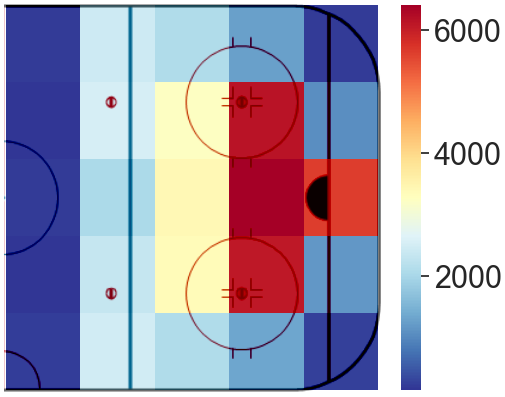
\includegraphics[scale=0.19]{figures/spatial_train_num_blend_crop.png}
    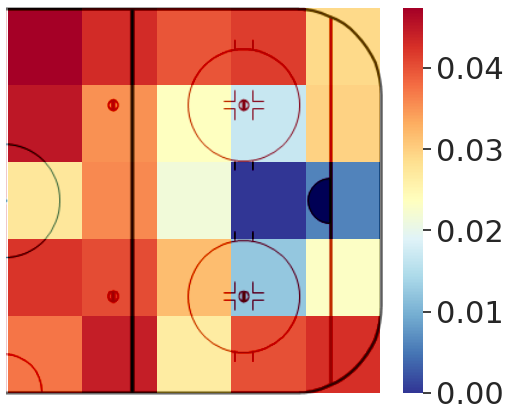
\includegraphics[scale=0.19]{figures/spatial_std_diff_blend_crop.png}
    % \end{minipage}
    % \vspace{-0.3in}
    \captionsetup{width=.95\linewidth}
    \caption{We discretize the ice hockey rink into 5$\times$5 regions. For each region, the {\it left} heatmap shows the number of shots in the {\it training dataset}, and the {\it right} heatmap shows the Mean Absolute Error (MAE) between the estimated and the real aleatoric uncertainty for shot values in the {\it testing dataset}. We observe a negative correlation (-0.761) between the density and the MAE across these regions.}
    \label{fig:spatial-uncertainty}
    \vspace{-0.2in}
    % \vspace{-0.1in}
    % \end{minipage}
    % \begin{minipage}[t]{0.5\textwidth}
    % 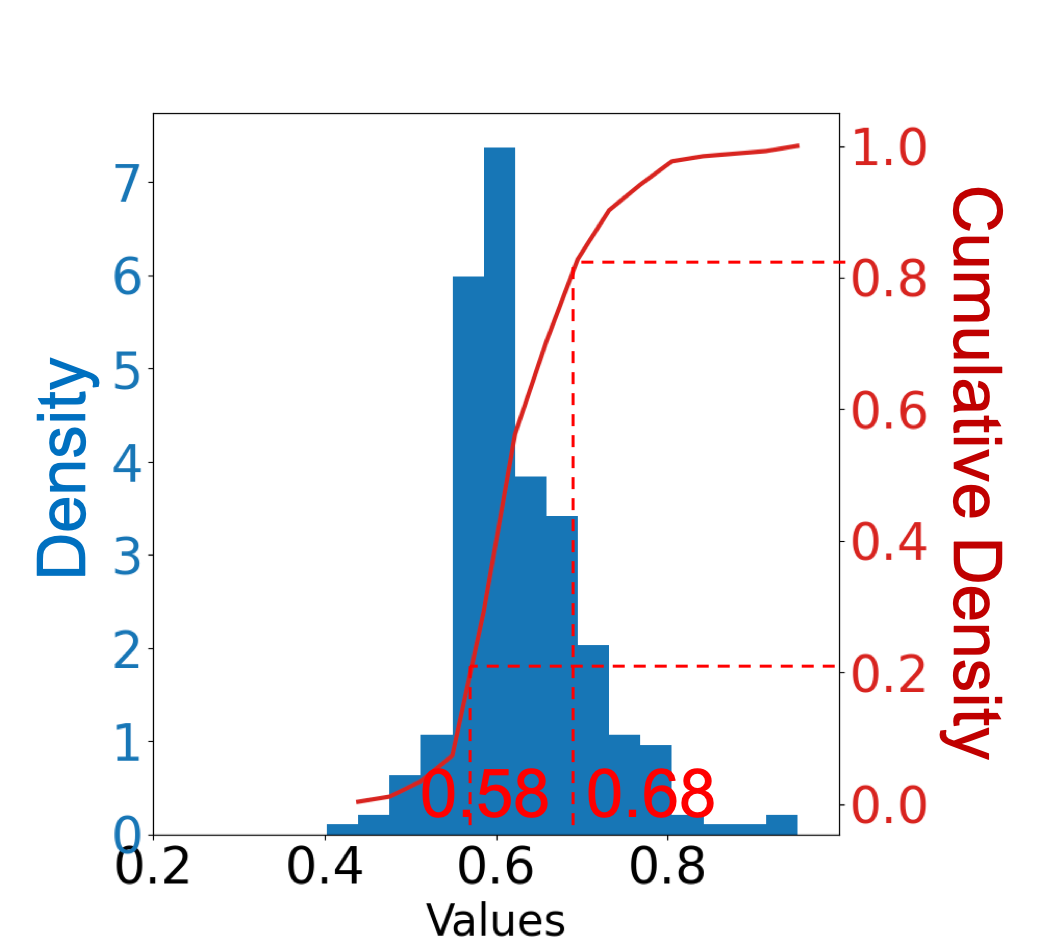
\includegraphics[scale=0.18]{figures/density_idx_7_XCoord_85.69_YCoord_-21.88_marked.png}
    % 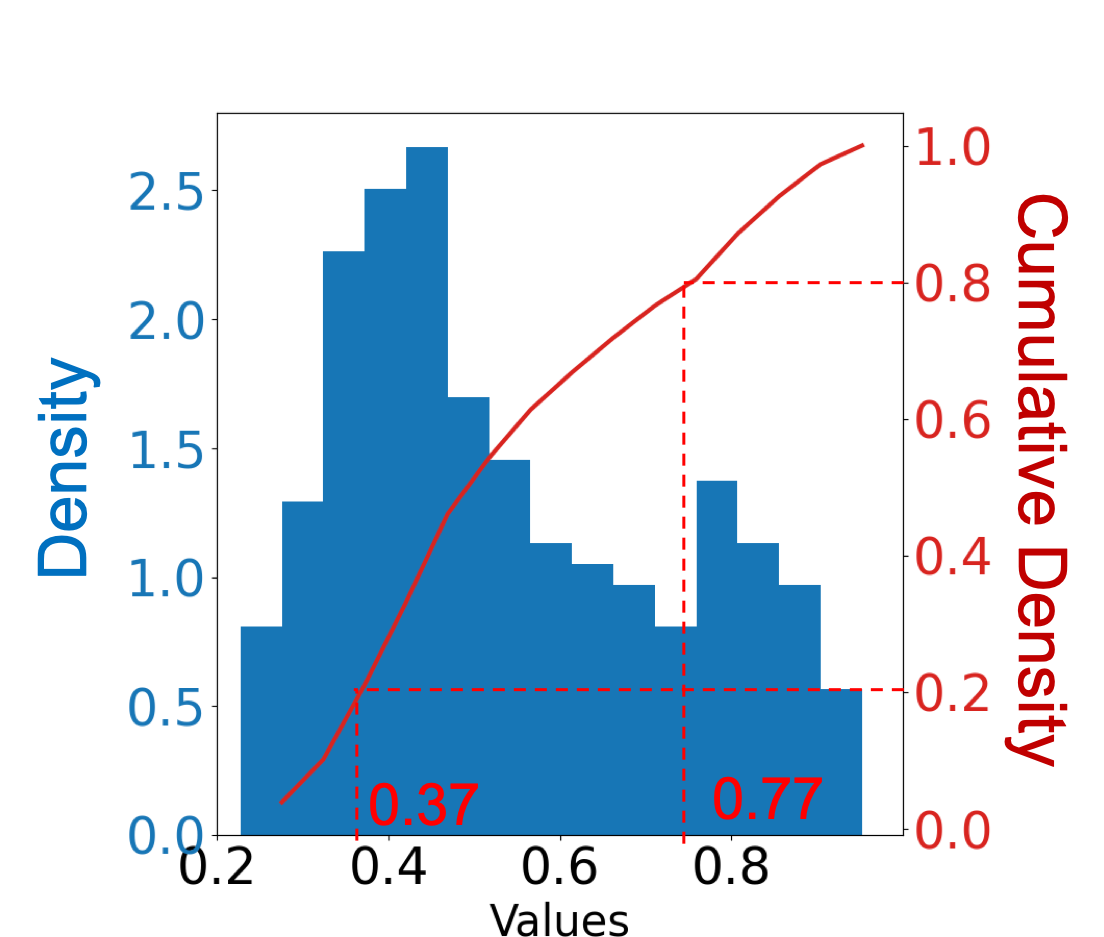
\includegraphics[scale=0.18]{figures/density_idx_21_XCoord_74.75_YCoord_-0.25_marked.png}
    % % \vspace{-0.1in}
    % % \end{minipage}
    % \captionsetup{width=.95\linewidth}
    % \caption{The next-goal distributions of two shots under different contexts. Both distributions have a similar expectation (around 0.6), but the first shot is less risky than the latter shot since the first shot has 1) a larger risk-averse estimate (when $c=0.8$, $0.58 > 0.37$) and 2) a smaller risk-seeking estimate (when $c=0.2$, $0.68 < 0.77$). \textcolor{blue}{move this plot above?}}
    % \label{fig:distribution-of-shot-returns}
    % % \vspace{-0.15in}
    % \end{minipage}
\end{wrapfigure}
\paragraph{Measuring Risk.} We measure the risk of a player's movement with the aleatoric uncertainty since modeling the intrinsic stochasticity of the game dynamics is consistent with the goal of sports analytics.
However, as Figure~\ref{fig:spatial-uncertainty} shows, when we quantify the aleatoric uncertainty with predictions from distributional RL, the performance is influenced by the density of input samples (i.e., OoD samples have a lower accuracy). 
% This influence can become more apparent with a distributional shift between training and testing data.

An effective approach to verify whether $\hat{Z}_{\agentIndex}(\state,\action)$ accurately captures the true aleatoric uncertainty is to check the epistemic uncertainty for each input data $(\state,\action)$~\cite{Mukhoti2021Uncertainty}: 1) a high input density ($p(\cdot|\condition)\geq\epsilon$) indicates low epistemic uncertainty,
(i.e., $(\state,\action)$ is inD)
and we can trust the aleatoric uncertainty estimated by distributional RL. 2) a low input density ($p(\cdot|\condition)<\epsilon$) indicates high epistemic uncertainty (i.e., the input is OoD, and we do not use the model prediction). In practice, $\epsilon$ is determined based on the validation dataset.

\noindent\textbf{Risk-Sensitive Action Impact.}
The {\it impact} $\impact(\state,\action)$ measures how much an action $\action$ changes the future return of a player's team. In terms of the value function, this is the change in action value due to a player’s movement. 
% \textcolor{blue}{The impact can be visualized as the difference between successive points in the action-value ticker (Figure xxx).} 
Previous works~\cite{Routley2015Markov,Liu2018DRL,Decroos2019Actions} computed the impact with the expected next-goal return $Q(\state_{t},\action_{t})=\expect[Z(\state_{t},\action_{t})]$. $Q(\cdot)$ does not take into account the inherent variability of the returns and thus cannot estimate the risk of an action. 
% Actions with similar expected returns can have significantly different risk-sensitive estimates. 
To understand how players respond to risk, we propose a Risk-sensitive Game Impact Metric (\system) based on $\hat{Z}_{\agentIndex}(\state,\action)$ and $p(\cdot|\condition)$:
% \vspace{-0.03in}
\begin{align}
    &\impact_{\agentIndex}(\state_{t+1},\action_{t+1},\confidence)=\big[\hat{Z}^{\confidence}_{\agentIndex}(\state_{t+1},\action_{t+1})-
    % 1/\gamma \expect_{\state_{t},\action_{t}}[
    \hat{Z}^{\confidence}_{\agentIndex}(\state_{t},\action_{t})\big]\mathbb{I}_{p(\cdot|\condition)\geq\epsilon}
    % ]
    \nonumber\\
    &\sys_{\playerId}(\confidence)=\sum_{(\state,\action)\in\dataset^{\prime}}n(\state,\action,\playerId)\times\impact_{\agentIndex}(\state,\action,\confidence)\label{eqn:RIGIM}
    \vspace{-0.1in}
\end{align}
where $\confidence\in[0,1]$ is the confidence level, $Z^{\confidence}$ denotes the $(1-\confidence)^{th}$ quantile in $Z(\cdot)$ and $n(\state,\action,\playerId)$ denotes the number of times that a player $\playerId$ performs action $\action$ at a state $\state$ in the testing dataset $\dataset^{\prime}$. We omit the term $\reward_t$ since $\reward_{t}=0$ except at scoring step $T$, and $\state_{T}$ is the terminal state of a scoring episode.
% (i.e., $\state_{T+1}$ does not exist). 
% In the expectation term, only the data points $\state_{t},\action_{t}$ whose next state is $\state_{t+1}$ will be measured. 
$\impact(\cdot)$ can either be 1) risk-averse (with a large $\confidence$), with better sensitivity to bad outcomes or 2) risk-seeking (with a small $\confidence$), with better sensitivity to positive outcomes.
%\vspace{-0.05in}
\subsection{Case Study: Player Ranking in Testing Games}
%\vspace{-0.05in}
We rank players according to their \system scores in the NHL testing games (see the experiment setting in Section~\ref{Sec:experiment}) at different confidence levels. 
Tables~\ref{table:player-ranking-0.2} and~\ref{table:player-ranking-0.8} illustrates how a domain expert could use our method to gain insight into which types of players exhibit different risk-taking behavior.
Table~\ref{table:player-ranking-0.2} shows a {\it risk-seeking} ranking (confidence $\confidence=0.2$),  which favors offensive players (e.g., Centres (C)) with strong scoring ability. Aleksander Barkov, who scores the most points in these games, is captured by this ranking. When we set confidence $\confidence$ to 0.8, Table~\ref{table:player-ranking-0.8} shows a {\it risk-averse} ranking which highlights players in defensive positions (e.g., Defensive (D)). John Klingberg, the defenseman with the most assists, is listed in the top-10 players. 
We believe the differences between Tables 1 and 2 can be explained by the fact that RiGIM is correlated with the types of actions a player performs. Intuitively, in ice-hockey, some actions are more risk-seeking (shot) in terms of scoring while other actions are risk-averse (carry or pass). In general, players in the backcourt (e.g., defensemen) are more likely to perform risk-averse actions that have smaller variance on the scoring chances.


% \textcolor{blue}{add a soccer ranking?}
% We find the risk-seeking players generally score more goals that the risk-averse player, which is consitant with 

% according to their performance in the testing games. 
\begin{table}[htbp]
\centering
\vspace{-0.1in}
\begin{minipage}[t]{0.5\textwidth}
\captionsetup{width=.9\linewidth}
\caption{Top 10 players with confidence 0.2.}\label{table:player-ranking-0.2}
\resizebox{1\textwidth}{!}{
\begin{tabular}{ccccccc}
\toprule
Player Name  & Position & Team  & P & A & G & \sys \\ \hline
Jonathan Toews & C & CHI & 10 & 5 & 5 & 14.72\\ 
Anze Kopitar & C & LAK & 12 & 9 & 3 & 14.55\\ 
Vincent Trocheck & C & FLA & 8 & 5 & 3 & 14.02\\ 
Tomas Hertl & C & SJS & 12 & 8 & 4 & 13.97\\ 
John Tavares & C & TOR & 12 & 3 & 9 & 13.92\\ 
Tyler Seguin & C & DAL & 18 & 12 & 6 & 13.71\\ 
Leon Draisaitl & C & EDM & 16 & 8 & 8 & 13.16\\ 
Aleksander Barkov & C & FLA & 19 & 14 & 5 & 12.63\\ 
Sean Couturier & C & PHI & 11 & 6 & 5 & 12.62\\ 
Nathan MacKinnon & C & COL & 12 & 6 & 6 & 12.48\\ 
\bottomrule
\end{tabular}
}
\end{minipage}%
\begin{minipage}[t]{0.5\textwidth}
\centering
\captionsetup{width=.9\linewidth}
\caption{Top 10 players with confidence 0.8.}\label{table:player-ranking-0.8}
\resizebox{0.97\textwidth}{!}{
\begin{tabular}{ccccccc}
\toprule
Player Name  & Position & Team  & P & A & G & \sys \\ \hline
Radek Faksa & C & DAL & 6 & 3 & 3 & 2.74\\ 
Leon Draisaitl & C & EDM & 16 & 8 & 8 & 2.51\\ 
John Klingberg & D & DAL & 10 & 9 & 1 & 2.46\\ 
Esa Lindell & D & DAL & 3 & 1 & 2 & 2.29\\ 
Connor McDavid & C & EDM & 18 & 11 & 7 & 2.23\\ 
Tomas Hertl & C & SJS & 12 & 8 & 4 & 1.93\\ 
Miro Heiskanen & D & DAL & 5 & 3 & 2 & 1.86\\ 
Elias Pettersson & C & VAN & 8 & 6 & 2 & 1.79\\ 
Tyler Seguin & C & DAL & 18 & 12 & 6 & 1.78\\ 
Roope Hintz & LW & DAL & 11 & 7 & 4 & 1.77\\ 
\bottomrule
\end{tabular}
}
\end{minipage}
\vspace{-0.1in}
\end{table}

\section{Empirical Evaluation}\label{Sec:experiment}

\noindent\textbf{Dataset.} 
Our experiments utilize both a {\it ice-hockey} and a {\it soccer} dataset from the National Hockey League (NHL) and major European soccer leagues, which contain 9,213,371 events, covering 195 teams, 4,172 games, and 6,513 players. These datasets consist of events around the ball. Each event records the identity and action of the player possessing the ball, with time stamps and features of the game context (see all the game features in Appendix A.1). To the best of our knowledge, this is the {\it most extensive study for player evaluation}. Note that we {\it do not utilize virtual environments} like Atari~\cite{bellemare2013arcade} or Mujoco~\cite{Todorov2012Mujoco} because 1) the dynamics in these environments are deterministic without uncertainty to be modeled and 2) this paper mainly studies sports games that have stochastic dynamics~\cite{schwartz2017handbook}, which are valid test-beds for our method.

\noindent\textbf{Experiment Settings.} We divide the dataset into a training set (80\%), a validation set (10\%), and a testing set (10\%) according to game dates, so that games in the testing set happened after the games in the training and validation set. To predict the action values in the testing games, the metric must remain robust to OoD data points.
% \textcolor{blue}{is there a way to prove there are OoD datapoints, I guess some game statistics will help.} 
We report the results averaged over 5 independent runs. 

\noindent\textbf{Comparison Methods.} We employ an ablation design that iteratively removes parts from \system.  {\bf GIM} removes the uncertainty estimator by directly using a Deep Recurrent Q-Network for estimating action values~\cite{Liu2018DRL}. {\bf T0-GIM} removes the recurrent model and uses a Deep Q-Network (DQN) for the value function. We then replace the RL framework with a supervised learning framework for estimating action values by following {\bf VAEP}~\cite{Decroos2019Actions}. Instead of using function approximators, {\bf Scoring Impact (SI)}~\cite{Routley2015Markov} implements the tabular-based value iteration algorithm for computing action values from discretized spatial and temporal features. {\bf Expected-Goal (EG)} metric directly uses the expected action values instead of impact values for measuring player performance. The last 
% two
metric {\bf  Plus-Minus ($+/-$)}
% and {\bf Win Above Replacement (WAR)} are 
is based on game statistics and measures the goal-gain with and without the player on court. We summarize these metrics in Table~\ref{table:summary-baseline}.

\newcommand{\xmark}{\ding{55}}%
\newcommand{\cmark}{\ding{51}}
\begin{wrapfigure}{r}{0.5\textwidth}
\centering
\vspace{-0.25in}
\captionof{table}{A summary of the baseline Methods for player evaluation.}\label{table:summary-baseline}
\vspace{-0.1in}
\resizebox{0.5\textwidth}{!}{
    \begin{tabular}{ccccccc}
    \toprule
    Method & \begin{tabular}[c]{@{}l@{}}Risk-\\ Aware\end{tabular} & \begin{tabular}[c]{@{}l@{}}History-\\ Aware\end{tabular} & \begin{tabular}[c]{@{}l@{}}RL-\\Based\end{tabular} & \begin{tabular}[c]{@{}l@{}}Continuous\\ Feature\end{tabular} &
    \begin{tabular}[c]{@{}l@{}}Impact-\\Based\end{tabular} &
    \begin{tabular}[c]{@{}l@{}}Context-\\ Aware\end{tabular} \\ \hline
    $+/-$ & \xmark  & \xmark  & \xmark   & \xmark   & \xmark  & \xmark  \\
    % WAR & \xmark  & \xmark  & \xmark   & \xmark   & \xmark  & \xmark  \\
    EG & \xmark  & \xmark  & \xmark   & \xmark   & \xmark  & \cmark \\
    SI & \xmark  & \xmark  & \xmark   & \xmark   & \cmark  & \cmark \\
    VAEP & \xmark  & \cmark  & \xmark   & \cmark  & \cmark  & \cmark \\
    T0-GIM & \xmark  & \xmark  & \cmark   & \cmark  & \cmark  & \cmark \\
    GIM & \xmark  & \cmark  & \cmark   & \cmark  & \cmark  & \cmark \\
    % Na-\system & \cmark  & \cmark  & \cmark   & \cmark  & \cmark  & \cmark \\ 
    \bottomrule
    \end{tabular}
    \vspace{-0.2in}
}
\end{wrapfigure}

To study how well SP-CNF boosts model performance, we compare 1) a Gaussian Discriminant Analysis {\bf (GDA)-\system} metric that replaces SP-CNF with GDA~\cite{Mukhoti2021Uncertainty}, and 2) a Naive {\bf (Na)-\system} metric that removes the epistemic uncertainty estimator 
and uses all the predicted distributions to compute players' impact (see Appendix A.2 and A.3 for more details.).


\subsection{Player Evaluation Performance: Correlations with Standard Measures}

We follow~\cite{Liu2018DRL,Luo2020IRL} and compute the correlations between player ranking metrics and standard measures on the testing games in a game season, because 1) the player (or agent) evaluation task has no ground-truth labels or rewards to maximize, 2) the correlation to all measures (including penalty measures) can measure whether the metrics can form a comprehensive evaluation to a player's overall performance. We study 11 {\it success} measures for ice hockey and 8 {\it success} measures for soccer. To make the results more comprehensive, we also add 5 {\it penalty measures}. The studied measures
are popular measures from the NHL and soccer statistics websites\footnote{\url{http://www.nhl.com/stats/skaters} and  \url{https://www.whoscored.com/statistics}}. Following the popular risk-measures like Conditional Value at Risk (CVaR), we treat $\confidence$ as a hyper-parameter.
Since the comparison methods are expectation-based metrics, we study the options of 1) setting the confidence level ($\confidence$) of \system to 0.5 for a fair comparison 2) empirically determining $\confidence$ with the validation set ($\confidence^{*}=0.34$ and $0.49$ for the ice hockey and soccer datasets). The risk-sensitive results are shown in Section~\ref{subsec:risk-sensitive-results}.


Tables~\ref{table:Correlations-ice-hcokey} and~\ref{table:Correlations-soccer} show the average correlations in 5 independent runs on the testing dataset (see Tables C.1 and C.2 in Appendix for the complete mean $\pm$ standard deviation results). \system achieves the highest correlations with 14 out of 19 success measures and the smallest correlations with 3 out of 5 penalty measures in ice hockey and soccer games. This observation shows that \system is a comprehensive metric that can detect both the positive and the negative influence of a player. If we remove SP-CNF or replace it with other uncertainty estimators, most correlations become weaker except for the correlations with the SHP and SHG measures. This is because SHP and SHG rarely happen in a season (scoring with fewer players on ice is difficult). SP-CNF detects this phenomenon and assigns small densities to these rare events. \system filters the event with a small density (see Equation~\ref{eqn:RIGIM}), which might cause the loss of information and make its correlation with SHP and SHG less significant.
SI correlates well with goal measures (Goals and Game Winning Goals) but has relatively poor correlations with other measures. This is because assigning an adequate value for {\em all} actions, including those with only intermediate effects on goal scoring, requires credit propagation over longer sequences, where neural nets are better at credit propagation than discretizing and using a tabular representation.
For other risk-neutral methods, their performance is generally less satisfying when compared with risk-aware methods, especially for the $+/-$ metric, which shows the importance of capturing risk and modeling the context features.
\begin{table}[htbp]
    \centering
    \vspace{-0.1in}
    \caption{Correlations with standard measures in the \textbf{ice hockey} games. The {\it success} measures are assist, goal, Game Winning Goal (GWG), Overtime Goal (OTG), Short-handed Goal (SHG), Power-play Goal (PPG), Point (P), Short-handed Point (SHP), Power-play Point (PPP), Time On Ice (TOI), and Shots (S). The {\it penalty} measure is Penalty Minute (PIM).}
    \resizebox{1\textwidth}{!}{
    \begin{tabular}{lccccccccccc:c}
    \toprule
         Methods & Assist & Goal & GWG & OTG & SHG & PPG & Point & SHP & PPP & TOI & S & PIM  \\\hline
         $+/-$ & 0.181 & 0.189 & 0.187 & 0.028 & 0.071 & 0.063 & 0.206 & 0.119 & -0.071 & 0.021 & 0.038 & -0.014\\
         EG & 0.239 & 0.303 & 0.264 & 0.130 & -0.053 & 0.163 & 0.322& 0.023& 0.226 & 0.153 & 0.534 & \underline{-0.112}\\
         SI & 0.237 & {\bf 0.596} & {\bf 0.409} & 0.123 & 0.095 & 0.351 & 0.452 & 0.066 & 0.274 & 0.224 & 0.405  & 0.138\\
         VAEP & 0.238 & 0.454 & 0.225 & 0.06 & 0.053 & 0.326 & 0.382 & -0.0 & 0.321 & 0.086 & 0.362 & 0.027\\
         T0-GIM & 0.397 & 0.394 & 0.139 & 0.16 & 0.151 & 0.216 & 0.455 & 0.153 & 0.295 & 0.356 & 0.387  & 0.058\\
         GIM & 0.456 & 0.408 & 0.167 & 0.158 & 0.134 & 0.246 & 0.501 & 0.137 & 0.345 & 0.395 & 0.431 & 0.061\\\hdashline
         Na-\sys({0.5}) & 0.593 & 0.476 & 0.223 & 0.173 & {\bf 0.152} & 0.313 & 0.625 & {\bf 0.175} & 0.453 & 0.597 & 0.611 & 0.115\\
         GDA-\sys({0.5}) & 0.591 & 0.475 & 0.221 & 0.174 & {\bf 0.152} & 0.315 & 0.623 & 0.174 & 0.452 & 0.593 & 0.609 & 0.113\\
         \sys({0.5}) & { 0.675} & 0.477 & 0.266 & { 0.184} & 0.11 & { 0.355} & { 0.678} & 0.141 & { 0.529} & { 0.68} & { 0.7} & 0.146 \\
         \sys({$\confidence^{*}$}) & {\bf 0.68} & 0.477 & 0.269 & {\bf 0.187} & 0.107 & {\bf 0.357} & {\bf 0.681} & 0.141 & {\bf 0.531} & {\bf 0.685} & {\bf 0.707} & 0.147\\
    \bottomrule
    \end{tabular}
    }
    \vspace{-0.05in}
    \label{table:Correlations-ice-hcokey}
\end{table}
\begin{table}[htbp]
    \centering
    \vspace{-0.1in}
    \caption{Correlations with standard measures in the \textbf{soccer} dataset. The {\it success} measures are goal, assist, Shots per Game (SpG), Pass Success percentage (PS\%), Key Passes (KeyP), Dribbles (Drb), Crosses and (being) Fouled. The {\it penalty} measures are Yellow (Yel) and Red Card Received, Offsides (Off) and Own Goals (OwnG).}
    \resizebox{1\textwidth}{!}{
    \begin{tabular}{lcccccccc:cccc}
    \toprule
    % &\multicolumn{8}{c:}{Positive Measures} & \multicolumn{4}{c}{Negative Measures} \\\hline\hline
         Methods& Goal & Assist & SpG & PS\% & KeyP & Drb & Crosses & Fouled & Yel & Red & Off & OwnG \\\hline
         $+/-$ & 0.284 & 0.318 & 0.199 & {\bf 0.288} & 0.218 & 0.119 & 0.017 & 0.035 & 0.001 & -0.069 & 0.053 & -0.001 \\
         EG & 0.422 & 0.173 & 0.328 & 0.164 & 0.278 & 0.013 & 0.040 & -0.026 & 0.534 & 0.034 & -0.124 & -0.008 \\
         SI &  0.585 & 0.153 & 0.438 & -0.140 & 0.052 & 0.050 & 0.216 & -0.065 & 0.114 & \underline{-0.089} & -0.249 & -0.102 \\
         VAEP & 0.093 & 0.290 & 0.121 & -0.111 & 0.116 & 0.059 & 0.082 & -0.00 & 0.024 & 0.133  & -0.055 & -0.051 \\
         T0-GIM & 0.614 & 0.455 & 0.715 & 0.148 & 0.472 & 0.431 & 0.161 & 0.355 & -0.007 & -0.027 & -0.346 & -0.168 \\
         GIM & 0.627 & 0.462 & 0.72 & 0.149 & 0.473 & 0.437 & 0.169 & 0.358 & -0.0 & -0.025 & -0.336 & -0.154 \\\hdashline
         Na-\sys({0.5})  & 0.646 & 0.507 & 0.741 & 0.144 & 0.503 & 0.445 & 0.177 & 0.391 & 0.101 & 0.007 & -0.309 & -0.144 \\
         GDA-\sys({0.5}) & 0.649 & 0.506 & 0.725 & 0.132 & 0.478 & 0.421 & 0.161 & 0.389 & 0.147 & 0.018 & -0.259 & -0.125  \\
         \sys({0.5}) & 0.671 & 0.577 & 0.756 & 0.181 & 0.574 & 0.530 & {\bf 0.239} & {\bf 0.448} & -0.092 & -0.039 & -0.451 &
         \underline{-0.185} \\
         \sys({$\confidence^{*}$}) & {\bf 0.682} & {\bf 0.583} & {\bf 0.757} & 0.186 & {\bf 0.575} & {\bf 0.531} & 0.238 & 0.446 & \underline{-0.101} & -0.042 & \underline{-0.455} & -0.184 \\
    \bottomrule
    \end{tabular}
    }
    \vspace{-0.15in}
    \label{table:Correlations-soccer}
\end{table}
\subsection{Sensitivity to Risk: Correlations Conditioning on Different Confidence Levels}~\label{subsec:risk-sensitive-results}
% %\vspace{-0.05in}
We measure whether \system is sensitive to the risk by its correlations with the standard measures, where \system is conditioned on a specific confidence level $\confidence$ (from 0 to 1), for example, \sys$(c)$, which indicates with probability $\confidence$ that the players' impact should be at least \sys$(\confidence)$.

Figures~\ref{fig:risk-sensitivity-ice-hockey} and~\ref{fig:risk-sensitivity-soccer} show the correlations at different confidence levels for ice-hockey and soccer games. \system is sensitive to risk, in the sense that it has different correlations with standard measures at these confidence levels, whereas GIM, as a risk-neutral metric, is unaware of the risk, and thus its correlations remain unchanged. 
Compared to other baselines, our \system generally maintains higher correlations with success measures and lower correlations with penalty measures. The exceptions are the correlations with the SHP, SHG, and OTG. For the same reason as discussed above, SP-CNF may filter them during testing. 
We find when $\confidence$ becomes smaller, \sys$(\confidence)$ becomes risk-seeking, and thus achieves a higher correlation with success measures. However, the correlations drop when $\confidence$ approaches 0. This is because $\hat{Z}_{\agentIndex}^{0}$ denotes the estimates at the largest quantile level (see Equation~\ref{eqn:RIGIM}), which corresponds to the most optimistic estimation action value (i.e., label scoring for all the shots). The overly risk-seeking estimation can induce a mismatch between estimated values and game facts, and thus cannot reflect the real contributions of players.

\begin{figure*}[htbp]
\vspace{-0.1in}
    \begin{minipage}{0.01\textwidth}
    \centering
    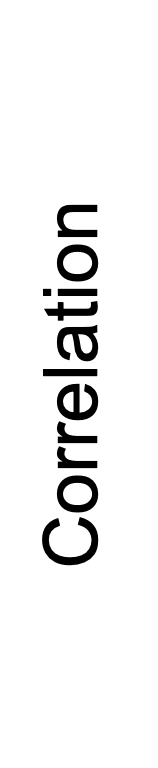
\includegraphics[scale=0.12]{figures/correlation_y_label.png}
    \end{minipage}
    \begin{minipage}{0.16\textwidth}
    \centering
    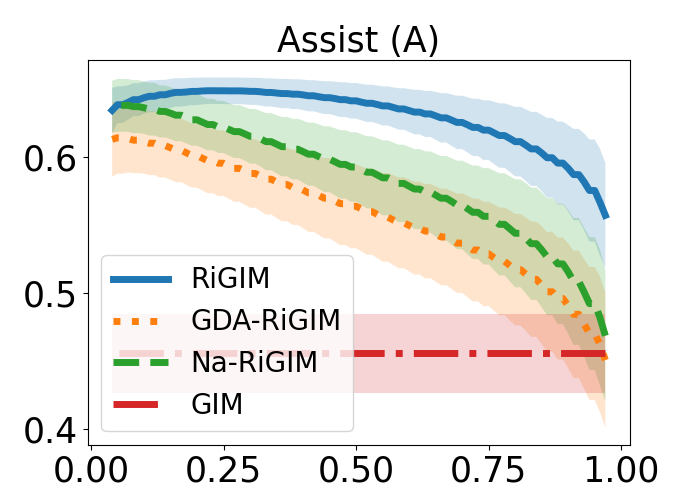
\includegraphics[scale=0.14]{figures/risk_curve_A_shadow.png}\par
    \vspace{-0.05in}
    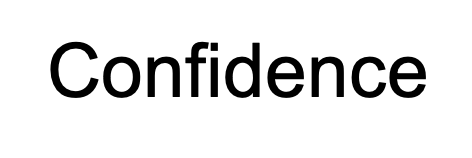
\includegraphics[scale=0.12]{figures/confidence_x_label.png}
    \end{minipage}
    \begin{minipage}{0.16\textwidth}
    \centering
    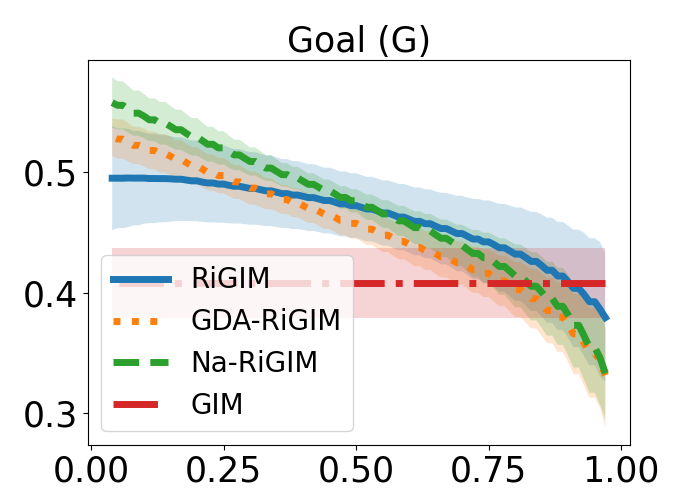
\includegraphics[scale=0.14]{figures/risk_curve_G_shadow.png}\par
    \vspace{-0.05in}
    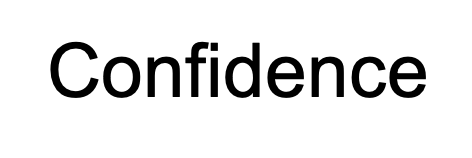
\includegraphics[scale=0.12]{figures/confidence_x_label.png}
    \end{minipage}
    \begin{minipage}{0.16\textwidth}
    \centering
    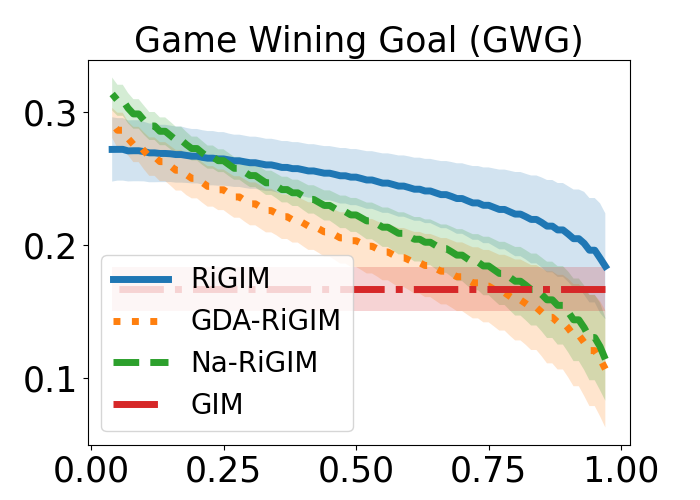
\includegraphics[scale=0.14]{figures/risk_curve_GWG_shadow.png}\par
    \vspace{-0.05in}
    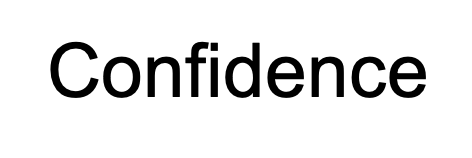
\includegraphics[scale=0.12]{figures/confidence_x_label.png}
    \end{minipage}
    \begin{minipage}{0.16\textwidth}
    \centering
    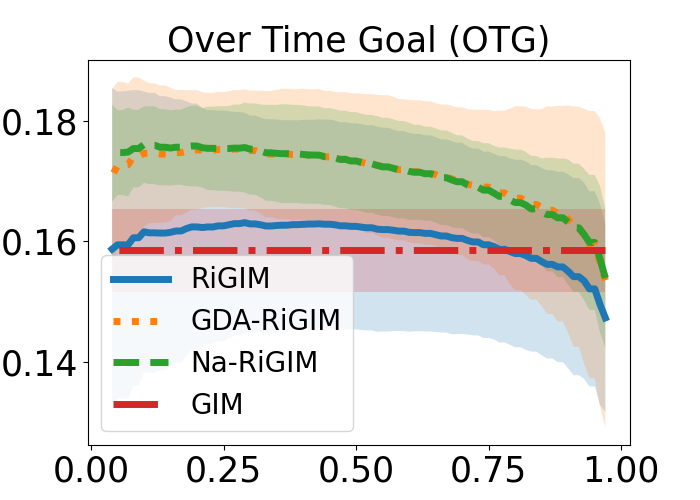
\includegraphics[scale=0.14]{figures/risk_curve_OTG_shadow.png}\par
    \vspace{-0.05in}
    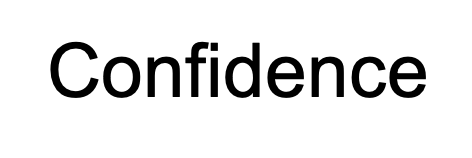
\includegraphics[scale=0.12]{figures/confidence_x_label.png}
    \end{minipage}
    \begin{minipage}{0.16\textwidth}
    \centering
    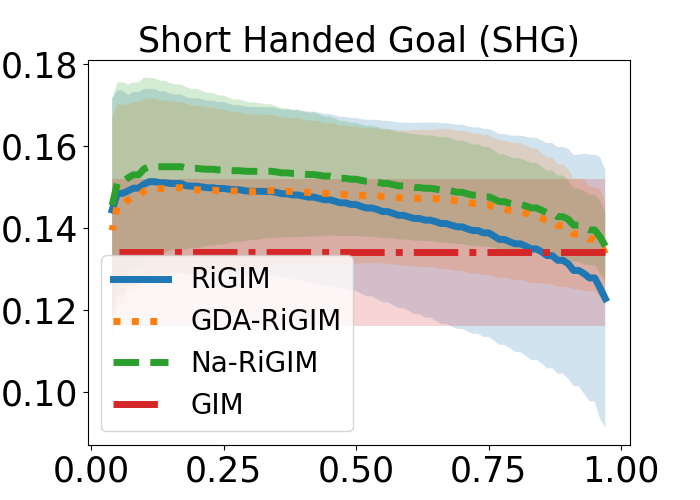
\includegraphics[scale=0.14]{figures/risk_curve_SHG_shadow.png}\par
    \vspace{-0.05in}
    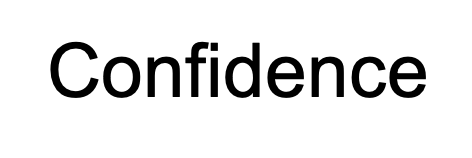
\includegraphics[scale=0.12]{figures/confidence_x_label.png}
    \end{minipage}
    \begin{minipage}{0.16\textwidth}
    \centering
    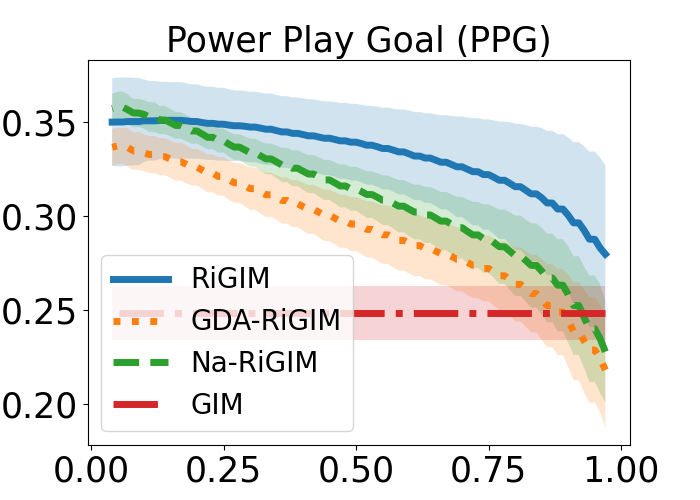
\includegraphics[scale=0.14]{figures/risk_curve_PPG_shadow.png}\par
    \vspace{-0.05in}
    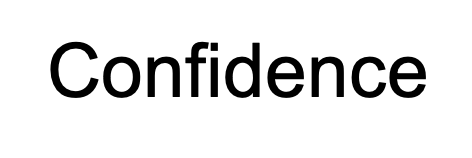
\includegraphics[scale=0.12]{figures/confidence_x_label.png}
    \end{minipage}
    \begin{minipage}{0.01\textwidth}
    \centering
    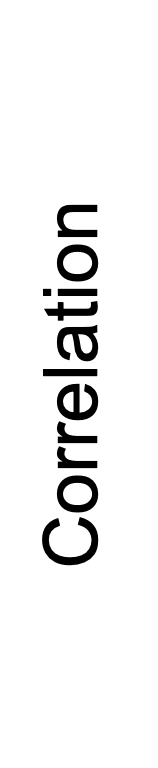
\includegraphics[scale=0.12]{figures/correlation_y_label.png}
    \end{minipage}
    \begin{minipage}{0.16\textwidth}
    \centering
    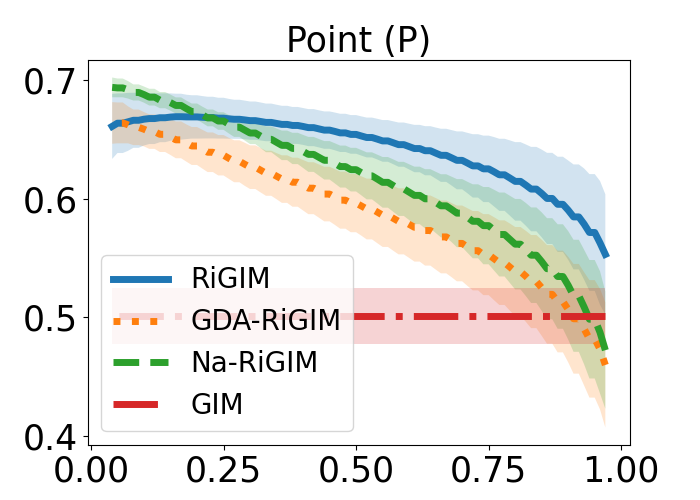
\includegraphics[scale=0.14]{figures/risk_curve_P_shadow.png}\par
    \vspace{-0.05in}
    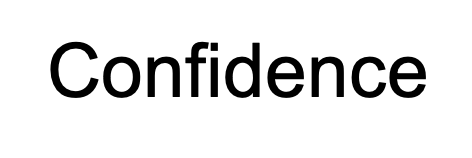
\includegraphics[scale=0.12]{figures/confidence_x_label.png}
    \end{minipage}
    \begin{minipage}{0.16\textwidth}
    \centering
    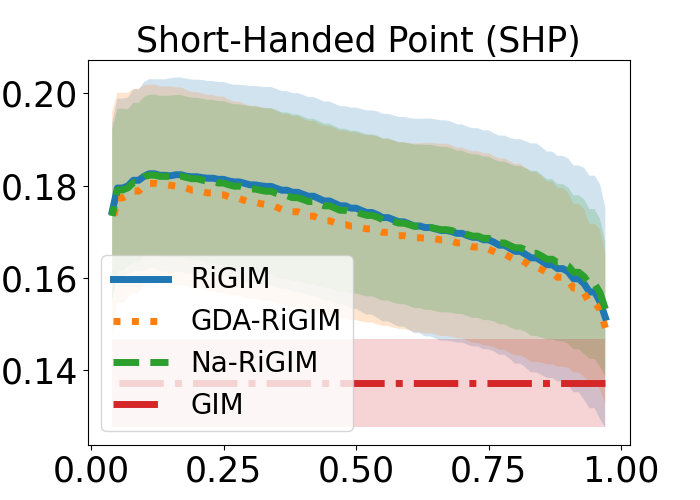
\includegraphics[scale=0.14]{figures/risk_curve_SHP_shadow.png}\par
    \vspace{-0.05in}
    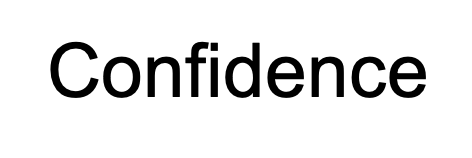
\includegraphics[scale=0.12]{figures/confidence_x_label.png}
    \end{minipage}
    \begin{minipage}{0.16\textwidth}
    \centering
    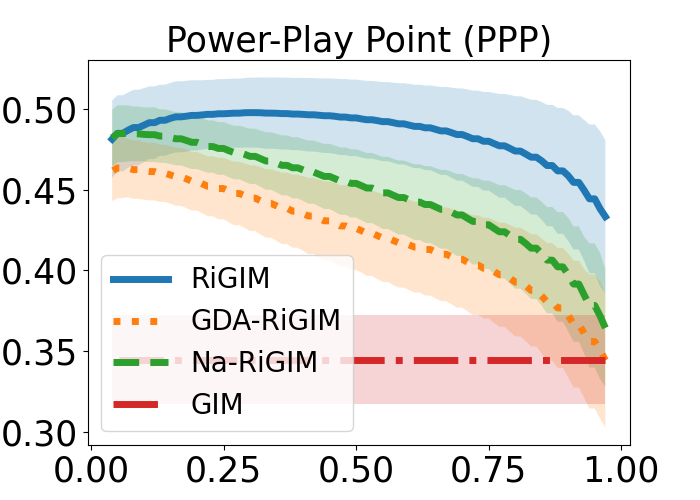
\includegraphics[scale=0.14]{figures/risk_curve_PPP_shadow.png}\par
    \vspace{-0.05in}
    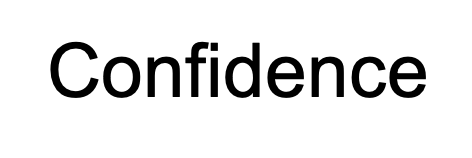
\includegraphics[scale=0.12]{figures/confidence_x_label.png}
    \end{minipage}
    \begin{minipage}{0.16\textwidth}
    \centering
    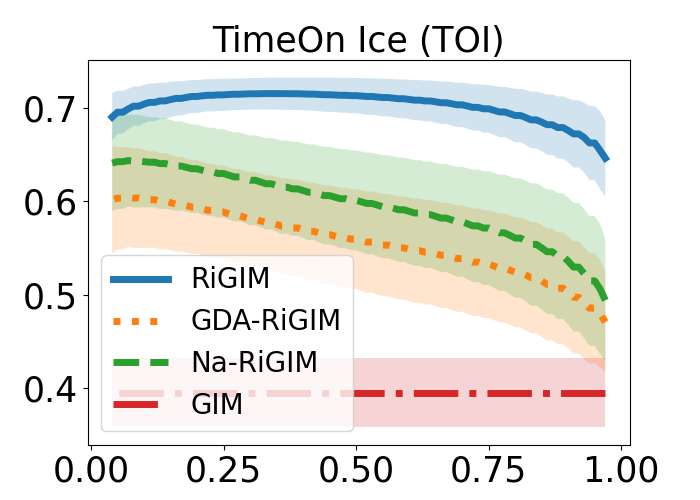
\includegraphics[scale=0.14]{figures/risk_curve_GP_shadow.png}\par
    \vspace{-0.05in}
    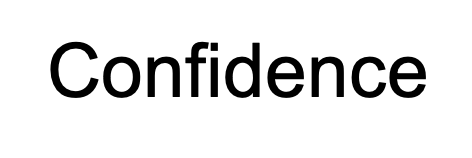
\includegraphics[scale=0.12]{figures/confidence_x_label.png}
    \end{minipage}
    \begin{minipage}{0.16\textwidth}
    \centering
    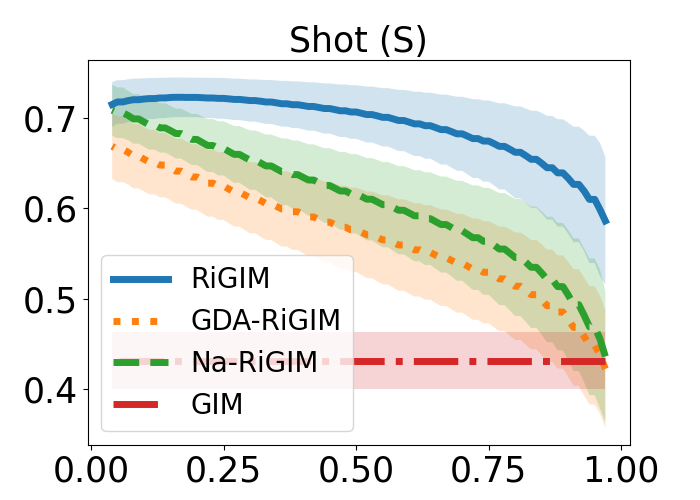
\includegraphics[scale=0.14]{figures/risk_curve_S_shadow.png}\par
    \vspace{-0.05in}
    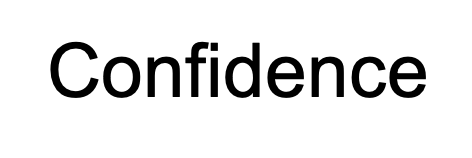
\includegraphics[scale=0.12]{figures/confidence_x_label.png}
    \end{minipage}
    \begin{minipage}{0.16\textwidth}
    \centering
    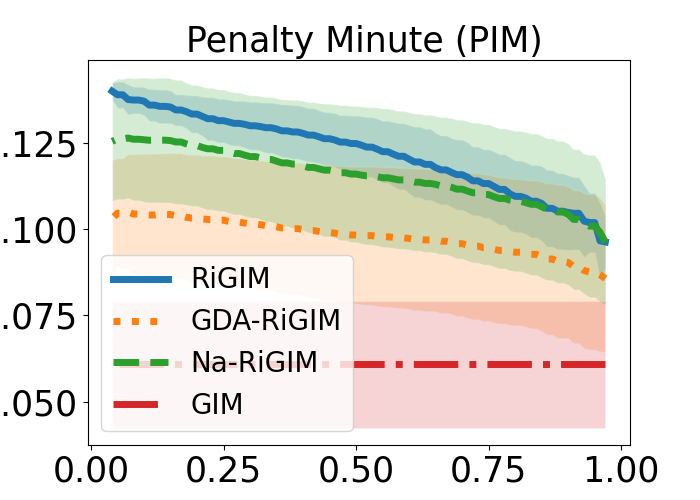
\includegraphics[scale=0.14]{figures/ice-hockey_risk_curve_PIM_shadow.png}\par
    \vspace{-0.05in}
    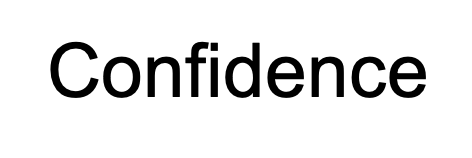
\includegraphics[scale=0.12]{figures/confidence_x_label.png}
    \end{minipage}
    % \par
    % \begin{center}
    % \vspace{-0.05in}
    % 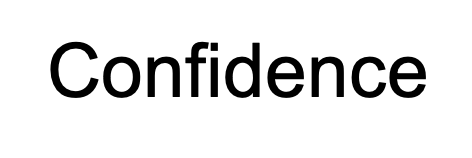
\includegraphics[scale=0.15]{figures/confidence_x_label.png}
    % \end{center}
    \vspace{-0.05in}
    \caption{Correlations (Mean $\pm$ standard deviation) with success measures (the first 11 plots) and penalty measures (the last plot) at different confidence levels in {\bf ice-hockey} games.}\label{fig:risk-sensitivity-ice-hockey}
    %\vspace{-0.2in}
\end{figure*}
\begin{figure*}[htbp]
    \begin{minipage}{0.01\textwidth}
    \centering
    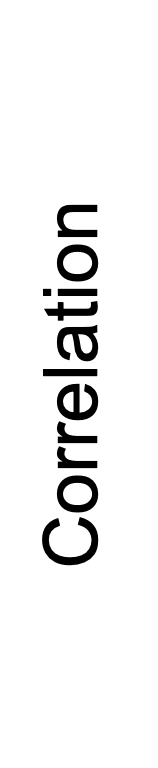
\includegraphics[scale=0.12]{figures/correlation_y_label.png}
    \end{minipage}
    \begin{minipage}{0.16\textwidth}
    \centering
    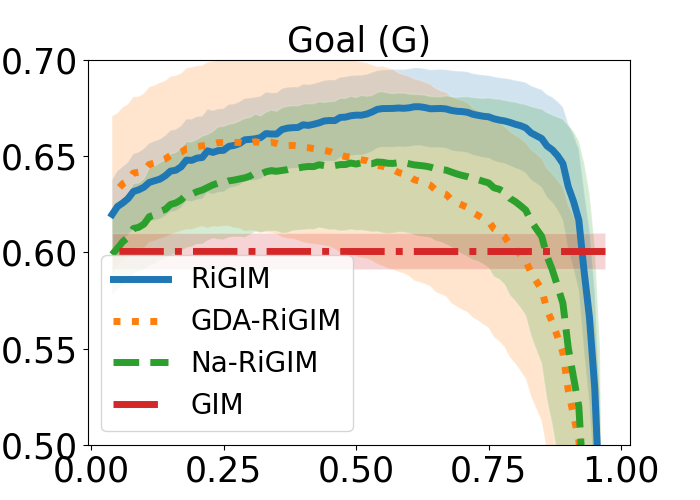
\includegraphics[scale=0.14]{figures/soccer_risk_curve_Goals_shadow.png}\par
    \vspace{-0.05in}
    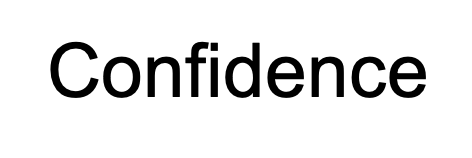
\includegraphics[scale=0.12]{figures/confidence_x_label.png}
    \end{minipage}
    \begin{minipage}{0.16\textwidth}
    \centering
    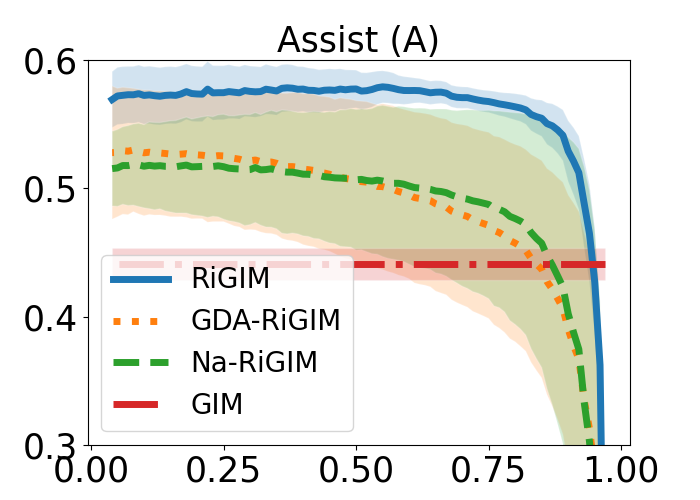
\includegraphics[scale=0.14]{figures/soccer_risk_curve_Assists_shadow.png}\par
    \vspace{-0.05in}
    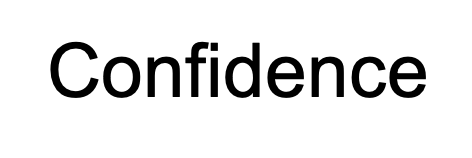
\includegraphics[scale=0.12]{figures/confidence_x_label.png}
    \end{minipage}
    \begin{minipage}{0.16\textwidth}
    \centering
    \includegraphics[scale=0.14]{figures/soccer_risk_curve_SpG_shadow.png}\par
    \vspace{-0.05in}
    \includegraphics[scale=0.12]{figures/confidence_x_label.png}
    \end{minipage}
    \begin{minipage}{0.16\textwidth}
    \centering
    \includegraphics[scale=0.14]{figures/soccer_risk_curve_PS_shadow.png}\par
    \vspace{-0.05in}
    \includegraphics[scale=0.12]{figures/confidence_x_label.png}
    \end{minipage}
    \begin{minipage}{0.16\textwidth}
    \centering
    \includegraphics[scale=0.14]{figures/soccer_risk_curve_KeyP_shadow.png}\par
    \vspace{-0.05in}
    \includegraphics[scale=0.12]{figures/confidence_x_label.png}
    \end{minipage}
    \begin{minipage}{0.16\textwidth}
    \centering
    \includegraphics[scale=0.14]{figures/soccer_risk_curve_Drb_shadow.png}\par
    \vspace{-0.05in}
    \includegraphics[scale=0.12]{figures/confidence_x_label.png}
    \end{minipage}
    \begin{minipage}{0.01\textwidth}
    \centering
    \includegraphics[scale=0.12]{figures/correlation_y_label.png}
    \end{minipage}
    \begin{minipage}{0.16\textwidth}
    \centering
    \includegraphics[scale=0.14]{figures/soccer_risk_curve_Crosses_shadow.png}\par
    \vspace{-0.05in}
    \includegraphics[scale=0.12]{figures/confidence_x_label.png}
    \end{minipage}
    \begin{minipage}{0.16\textwidth}
    \centering
    \includegraphics[scale=0.14]{figures/soccer_risk_curve_Fouled_shadow.png}\par
    \vspace{-0.05in}
    \includegraphics[scale=0.12]{figures/confidence_x_label.png}
    \end{minipage}
    \begin{minipage}{0.16\textwidth}
    \centering
    \includegraphics[scale=0.14]{figures/soccer_risk_curve_Yel_shadow.png}\par
    \vspace{-0.05in}
    \includegraphics[scale=0.12]{figures/confidence_x_label.png}
    \end{minipage}
    \begin{minipage}{0.16\textwidth}
    \centering
    \includegraphics[scale=0.14]{figures/soccer_risk_curve_Red_shadow.png}\par
    \vspace{-0.05in}
    \includegraphics[scale=0.12]{figures/confidence_x_label.png}
    \end{minipage}
    \begin{minipage}{0.16\textwidth}
    \centering
    \includegraphics[scale=0.14]{figures/soccer_risk_curve_Offsides_shadow.png}\par
    \vspace{-0.05in}
    \includegraphics[scale=0.12]{figures/confidence_x_label.png}
    \end{minipage}
    \begin{minipage}{0.16\textwidth}
    \centering
    \includegraphics[scale=0.14]{figures/soccer_risk_curve_OwnG_shadow.png}\par
    \vspace{-0.05in}
    \includegraphics[scale=0.12]{figures/confidence_x_label.png}
    \end{minipage}
    % \par
    % \begin{center}
    % %\vspace{-0.05in}
    % \includegraphics[scale=0.15]{figures/confidence_x_label.png}
    % \end{center}
    \vspace{-0.05in}
    \caption{Correlations (Mean $\pm$ standard deviation) with success measures (the first 8 plots) and penalty measures (the last 4 plots) at different confidence levels for in {\bf soccer} games.}\label{fig:risk-sensitivity-soccer}
    %\vspace{-0.2in}
\end{figure*}
\subsection{The Prediction Accuracy: Match Future Scoring Frequencies With Action-Values}
%\vspace{-0.05in}
We study how well the predicted action-value distributions match the real next-goal scoring frequencies under discrete game contexts. 
These game contexts are constructed by dividing the continuous state space into discrete bins. To calculate the empirical scoring frequency associated with each bin, we assign an observed state $\state$ to a bin $\bin$ according to the values of three discrete context features in the current observation: Manpower Differential, Goal Differential, and Period. The empirical and estimated scoring probabilities for a bin (with size $|\bin|$) are defined as follows:

a){ \it Empirical Scoring Chances}: for each $\state\in\bin$, we set $\goal_{\agentIndex}{(\state)} = 1$ if the observed scoring-episode containing state $\state$ ends with a goal by team $\agentIndex$. Then $\MakeUppercase{\goal}^{*}_{\agentIndex}(\bin) = \frac{1}{|\bin|}\sum_{\state \in \bin} \goal_{\agentIndex}(\state)$.

b){ \it Estimated Scoring Chances}: for each $\state\in\bin$, given $N$ samples from the calibrated distribution $z_{\agentIndex}(\state)\sim\hat{Z}_{\agentIndex}(\state,\action)\mathbb{I}_{p(\cdot|\condition)\geq\epsilon}$, the estimated chances are: $\hat{\MakeUppercase{\goal}}_{\agentIndex}(\bin) = \frac{1}{N|\bin|}\sum_{\state \in \bin} \sum_{n=1}^{N}z_{\agentIndex,n}(\state)$.
% \begin{table*}[htbp]
% \setlength{\tabcolsep}{4pt}
% % \setlength\extrarowheight{5pt}
% \centering
% \resizebox{1\textwidth}{!}{
% \begin{tabular}{l|ccc|ccc|ccc}
% \toprule
% \multirow{2}{*}{Context} & \multicolumn{3}{|c}{Manpower Differential} & \multicolumn{3}{|c}{Score Difference} & \multicolumn{3}{|c}{Period}\\ \cline{2-10} 
%  & Short-Handed & Even-Strength & Power-Play & -1 & 0 & 1 & Third & Second & First \\ \hline
% GIM & 0.115 $\pm$ 0.078 & 0.094 $\pm$ 0.082 & 0.099 $\pm$ 0.085 & 0.238 $\pm$ 0.122 & 0.105 $\pm$ 0.084 & 0.271 $\pm$ 0.059 & 0.095 $\pm$ 0.055 & 0.111 $\pm$ 0.086 & 0.114 $\pm$ 0.084 \\
% Na-RiGIM &  &  &  &  &  & \\
% GDA-RiGIM & 0.148 & 0.072 & 0.017 & 0.236 & 0.045 & 0.110 & 0.143 & 0.05 & 0.033 \\
% RiGIM &  &  &  &  &  &  \\ \bottomrule
% \end{tabular}
% }
% \end{table*}

\begin{table}[htbp]
\centering
%\vspace{-0.15in}
\caption{The difference between the empirical and the estimated scoring chances in different contexts. Results are averaged over 5 runs $\pm$ standard error.  $\uparrow (\downarrow)$ indicates that a difference is statistically greater (smaller) than the difference achieved by \system with p-value $\le 0.01$ according to the Wilcoxon signed rank test.}
\label{table:calibration-results}
\resizebox{1\textwidth}{!}{
\begin{tabular}{l|ccc:ccc}
\toprule
&\multicolumn{3}{c:}{Ice-Hockey} & \multicolumn{3}{c}{Soccer} \\\hline\hline
\begin{tabular}[c]{@{}c@{}}Manpower\\ Differential\end{tabular}& \begin{tabular}[c]{@{}c@{}}Short-\\ Handed\end{tabular} & \begin{tabular}[c]{@{}c@{}}Even-\\ Strength\end{tabular} & \begin{tabular}[c]{@{}c@{}}Power-\\ Play\end{tabular} & \begin{tabular}[c]{@{}c@{}}Short-\\ Handed\end{tabular} & \begin{tabular}[c]{@{}c@{}}Even-\\ Strength\end{tabular} & \begin{tabular}[c]{@{}c@{}}Power-\\ Play\end{tabular}\\\hline
GIM & 0.115 $\pm$ 0.078 $\downarrow$ & 0.094 $\pm$ 0.082 $\downarrow$ & 0.099 $\pm$ 0.085 $\downarrow$ & 0.211 $\pm$ 0.034 $\downarrow$ & {\bf 0.114} $\pm$ 0.05 $\uparrow$ & 0.199 $\pm$ 0.037 $\downarrow$ \\
Na-RiGIM & 0.133 $\pm$ 0.016 $\downarrow$ & 0.064 $\pm$ 0.016  $\downarrow$ & {\bf 0.013} $\pm$ 0.009 $\uparrow$ & 0.226 $\pm$ 0.019 $\downarrow$ & 0.136 $\pm$ 0.019  & 0.175 $\pm$ 0.028 $\downarrow$ \\
GDA-RiGIM & 0.148 $\pm$ 0.035 $\downarrow$ & 0.072 $\pm$ 0.029 $\downarrow$ & 0.017 $\pm$ 0.011  $\uparrow$ & 0.216 $\pm$ 0.022 $\downarrow$ & 0.151 $\pm$ 0.011 $\downarrow$ & 0.18 $\pm$ 0.013 $\downarrow$ \\
RiGIM & {\bf 0.080} $\pm$ 0.020 & {\bf 0.058} $\pm$ 0.008 & 0.047 $\pm$ 0.046 & {\bf 0.204} $\pm$ 0.005 & 0.133 $\pm$ 0.007 & {\bf 0.147} $\pm$ 0.033\\ \hline\hline
 Goal Differential & -1 & 0 & 1 & -1 & 0 & 1 \\\hline
GIM  & 0.238 $\pm$ 0.122 $\downarrow$ & 0.105 $\pm$ 0.084 $\downarrow$ & 0.271 $\pm$ 0.059 $\downarrow$ & 0.155 $\pm$ 0.047 $\downarrow$ & 0.155 $\pm$ 0.054 $\downarrow$ & 0.221 $\pm$ 0.049 $\downarrow$ \\
Na-RiGIM  & 0.238 $\pm$ 0.006 $\downarrow$ & 0.045 $\pm$ 0.015 $\downarrow$ & 0.108 $\pm$ 0.031 $\downarrow$ & 0.157 $\pm$ 0.02 & {\bf 0.104} $\pm$ 0.024 & 0.16 $\pm$ 0.017 $\downarrow$\\
GDA-RiGIM & 0.236 $\pm$ 0.007 $\downarrow$ & 0.045 $\pm$ 0.016 $\downarrow$ & 0.11 $\pm$ 0.027 & 0.165 $\pm$ 0.018 $\downarrow$ & 0.117 $\pm$ 0.017 $\downarrow$ & 0.175 $\pm$ 0.007 $\downarrow$\\
RiGIM & {\bf 0.193} $\pm$ 0.021 & {\bf 0.029} $\pm$ 0.015 & {\bf 0.092} $\pm$ 0.019 & {\bf 0.152} $\pm$ 0.008 & 0.109 $\pm$ 0.004 & {\bf 0.149} $\pm$ 0.013\\ \hline\hline
Period & 3 & 2 & 1 & 2$^{st}$ half
& 1$^{nd}$ half & N/A \\\hline
GIM & {\bf 0.095} $\pm$ 0.055 $\uparrow$ & 0.111 $\pm$ 0.086 $\downarrow$ & 0.114 $\pm$ 0.084 $\downarrow$ & {\bf 0.191} $\pm$ 0.037 $\uparrow$ & 0.104 $\pm$ 0.059 $\downarrow$ \\
Na-RiGIM  & 0.139 $\pm$ 0.018 & 0.044 $\pm$ 0.015 $\downarrow$ & 0.024 $\pm$ 0.015 $\downarrow$ & 0.237 $\pm$ 0.013 $\downarrow$ & 0.061 $\pm$ 0.03 $\downarrow$ \\
GDA-RiGIM & 0.143 $\pm$ 0.028 & 0.050 $\pm$ 0.025 $\downarrow$ & 0.033 $\pm$ 0.025 $\downarrow$ & 0.238 $\pm$ 0.012 $\downarrow$ & 0.059 $\pm$ 0.026\\
RiGIM & 0.143 $\pm$ 0.011 & {\bf 0.032} $\pm$ 0.005 & {\bf 0.014} $\pm$ 0.009  & 0.226 $\pm$ 0.011 & {\bf 0.058} $\pm$ 0.009\\ \bottomrule
\end{tabular}
}
\end{table}
%\vspace{-0.1in}
Table~\ref{table:calibration-results} shows the average absolute difference between $\hat{\MakeUppercase{\goal}}$ and $\MakeUppercase{\goal}^{*}$ based on 5 independent runs. 
We implement a Wilcoxon signed rank test~\cite{conover1999practical} to study whether the predictions from baseline methods are different from that of \system for all samples.
Our baselines are the learning-based action-values metrics for the context-aware evaluation. \system achieves a minimum distance in 12 out of 17 bins. This is because 1) FS-CNF outperforms GDA by computing a more accurate uncertainty estimator for filtering OoD states and 2) the distribution estimates contain richer information than expectation estimates, allowing $\Tilde{Z}(\cdot)$ to better match the scoring frequencies than $Q(\cdot)$. This observation is consistent with the findings in \cite{bellemare2017distributional}.

%\vspace{-0.05in}
\subsection{Limitations}~\label{subsec:limitations}
% %\vspace{-0.05in}
\noindent\textbf{A Study for Sports Games.} This work uses stochastic sports games as the testbeds for uncertainty estimation, but we argue the same methods can be easily migrated to other applications in stochastic environments such as autonomous driving or healthcare. Our approach of measuring aleatoric and epistemic risks can be adapted to offline RL for learning conservative policies.

\noindent\textbf{Evaluation Instead of Control.} Our method focuses on player evaluation instead of control. We believe both tasks are challenging with respect to different aspects. Evaluation requires the action values to accurately reflects an agent's real contribution to game-winning. An ideal evaluation metric can provide in-game predictions of game outcomes, which is important for the sports industry.
%\vspace{-0.05in}
\section{Conclusion and Future Work}
%\vspace{-0.05in}
In this paper, we designed an RL framework for quantifying the aleatoric uncertainty and the epistemic uncertainty from stochastic sports datasets. This framework enabled distributional RL and an FS-CNF model to estimate both uncertainties, with which we proposed a risk-sensitive evaluation metric \system. Empirical results show that \system correlates well with success measures and the correlation is sensitive to different risks. A direction of future work is to extend our model to other domains.

\begin{ack}
We acknowledge the funding from the Canada CIFAR AI Chairs program, and the support of the Natural Sciences and Engineering Research Council of Canada (NSERC). Resources used in this work were provided, in part, by the Province of Ontario, the Government of Canada through CIFAR, and companies sponsoring the Vector Institute     \url{https://vectorinstitute.ai/partners/}.
\end{ack}

\bibliographystyle{unsrt}
\bibliography{bibliography.bib}

\newpage

\section{Submission of papers to NeurIPS 2022}

\begin{enumerate}


\item For all authors...
\begin{enumerate}
  \item Do the main claims made in the abstract and introduction accurately reflect the paper's contributions and scope?
    \answerYes{}
  \item Did you describe the limitations of your work?
    \answerYes{Check Section~\ref{subsec:limitations}.}
  \item Did you discuss any potential negative societal impacts of your work?
    \answerYes{Check our Appendix D.}
  \item Have you read the ethics review guidelines and ensured that your paper conforms to them?
    \answerYes{}
\end{enumerate}


\item If you are including theoretical results...
\begin{enumerate}
\item Did you state the full set of assumptions of all theoretical results?
    \answerYes{Check Proposition 1 and the proof in Appendix B.}
\item Did you include complete proofs of all theoretical results?
    \answerYes{Check Proposition 1 and the proof in Appendix B.}
\end{enumerate}


\item If you ran experiments...
\begin{enumerate}
\item Did you include the code, data, and instructions needed to reproduce the main experimental results (either in the supplemental material or as a URL)?
    \answerYes{Check a detailed dataset introduction in Appendix A.1 and the instructions in Appendix A.2.}
\item Did you specify all the training details (e.g., data splits, hyperparameters, how they were chosen)?
    \answerYes{Check the experiment settings in Section~\ref{Sec:experiment} and Appendix A.2.}
\item Did you report error bars (e.g., with respect to the random seed after running experiments multiple times)?
    \answerYes{We use 5 random seeds for all experiments. Check the experiment settings in Section~\ref{Sec:experiment}, our experiment results and Table C.1 and C.2 in Appendix.}
\item Did you include the total amount of compute and the type of resources used (e.g., type of GPUs, internal cluster, or cloud provider)?
    \answerYes{Check Appendix A.4.}
\end{enumerate}


\item If you are using existing assets (e.g., code, data, models) or curating/releasing new assets...
\begin{enumerate}
\item If your work uses existing assets, did you cite the creators?
    \answerYes{There is not formal citation, so we add the link to the data source. Check our dataset introduction in Appendix A.1.}
\item Did you mention the license of the assets?
    \answerNA{There is no such licence that we can cite for this dataset.}
\item Did you include any new assets either in the supplemental material or as a URL?
    \answerNo{}
\item Did you discuss whether and how consent was obtained from people whose data you're using/curating?
    \answerYes{We have corporated on many projects.}
\item Did you discuss whether the data you are using/curating contains personally identifiable information or offensive content?
    \answerYes{Check our dataset introduction in Appendix A.1.}
\end{enumerate}


\item If you used crowdsourcing or conducted research with human subjects...
\begin{enumerate}
\item Did you include the full text of instructions given to participants and screenshots, if applicable?
    \answerNA{}
\item Did you describe any potential participant risks, with links to Institutional Review Board (IRB) approvals, if applicable?
    \answerNA{}
\item Did you include the estimated hourly wage paid to participants and the total amount spent on participant compensation?
    \answerNA{}
\end{enumerate}

\end{enumerate}


\end{document}